\chapter{HPS Analysis}
\label{chapter:hps:analysis}

A search for visibly-decaying \ac{dm} is not novel, many experiments have been purposed-built
for such a search; however, \ac{hps} is specially focused on \ac{dm} that decays
within shorter distances.
While \ac{hps} has previously searched for simple dark sectors
more similar to the benchmark model used within the \ac{ldmx} missing energy search \cite{hps-2016-displaced-vtx},
no \ac{dm} was found and the relatively longer decay lengths of this dark sector model
harmed the signal efficiency of the analysis and decreased the resulting sensitivity.
\cref{sec:hps:simps} introduced the idea of \ac{simp} \ac{dm} which has additional
interest for \ac{hps}.
Specifically, the increase in complexity of the \ac{dm} model slightly decouples the production
rate from the decay rate meaning the number of events where \ac{dm} is produced is not as tightly
connected to how displaced the particles are expected to be within the detector.
The downside of this decoupling is that some energy is lost to the production of the lighter
dark meson $\pi_D$ when the dark photon decays within the dark sector; however,
this also means \ac{hps} has not searched this regime since one of the key selections within
its previous displaced vertex search was requiring the total momentum of the vertex to be
near the beam energy instead of significantly below it.

With the samples presented in \cref{chapter:hps:dataset}, a search for \acp{simp} within the collected
data has been performed.
An additional, orthogonal category of data was introduced to be combined with prior work,
enabling higher sensitivity to a range of \ac{simp} parameter space.

\section{Signal Yield}
\label{sec:hps:signal-yield}

The expected signal yield is a crucial part of any kind of search analysis
and this one is no exception.
The prior search within \ac{ldmx} benefited from its missing momentum/energy technique
in this regard since the mixing strength $\epsilon$ is only connected to the scale of the signal
yield and not how the signal events would present themselves in the data.
In a visible search, the mixing strength also affects the decay length and thus a more intricate
signal yield estimate is required to account for the fact that changing $\epsilon$ not only changes
the magnitude but also changes which events are more likely to be observed within data.
In this analysis, we modify the expected signal yield calculation done previously by \ac{hps}
\cite{hps-2016-displaced-vtx} to accomodate the two viable decay channels within this \ac{simp} model.

The fundamental premise of this calculation is re-weighting events based on their decay length
so that they appear to have been drawn from a specific mixing strength's decay distribution.
Specifically, we integrate over a decay weighting factor multiplied by the signal efficiency
both as a function of the decay length in or to estimate the total signal yield for a specific
mixing strength.
The details of this calculation are presented in this section since they are relatively novel and
not presented fully in another publication; however, this does force me to deviate from my previous
commitment to few mathematical equations and jargony language.
Skip to \cref{sec:hps:recon-cat} if this detail does not interest you.

The magnitude of this estimate is set by the relationship between dark photon production cross section
and the radiative trident differential cross section\cite{bjorken-ap-rate:2009}.
\begin{equation}
  \sigma_{A'} = \epsilon^2\frac{3\pi}{2\alpha} m_{A'} \left.\frac{d\sigma_{\gamma^*}}{dm}\right|_{m=m_{A'}}
\end{equation}
Multiplying both sides by the dataset's luminosity then gives us event yields.
\begin{equation}
  N_{A'} = \epsilon^2\frac{3\pi}{2\alpha} m_{A'} \left.\frac{dN_{\gamma^*}}{dm}\right|_{m=m_{A'}}
\end{equation}
The complexity arises when we remember that specifically radiative tridents are not
directly observable -- they are intertwined with other standard processes that produce
the same outgoing particles (Bethe-Heitler tridents for example).
Thus, we estimate the radiative trident differential yield $dN_{\gamma^*}/dm$ by
modifying the observable trident differential yield $dN_{3e\mathrm{,CR}}/dm_\mathrm{reco}$ by
two simulation-derived factors.
The radiative fraction $f_\mathrm{rad}$ estimates the fraction of trident events
that originate from the radiative process.
\begin{equation}
  f_\mathrm{rad} = \frac{dN_{\gamma^*}}{dm} \bigg/ \frac{dN_{3e}}{dm_\mathrm{reco}}
\end{equation}
And the radiative acceptance times efficiency $A_\mathrm{rad}$ estimates the
fraction of trident events that are within the geometric acceptance of the detector
and pass the trigger and preselection requirements.
\begin{equation}
  A_\mathrm{rad} = \frac{dN_{3e,CR}}{dm_\mathrm{reco}} \bigg/ \frac{dN_{3e,\mathrm{gen}}}{dm_\mathrm{reco}}
\end{equation}
where CR stands for the Control Region in \Psum
(see \cref{sec:hps:analysis:variables} for the definition of this variable).
Thus, the expected yield of dark photons created within the detector
but not necessarily within its acceptance or passing selection requirements is
\begin{equation}
  N_{A'} = \epsilon^2\frac{3\pi}{2\alpha} m_{A'} 
    \frac{f_\mathrm{rad}}{A_\mathrm{rad}}
    \left.\frac{dN_{3e\mathrm{,CR}}}{dm_\mathrm{reco}}\right|_{m=m_{A'}}
\end{equation}
Both $f_\mathrm{rad}$ and $A_\mathrm{rad}$ use the event and vertex pre-selection before
any downstream analysis selections, so they are common amongst all potential analysis channels
that share this pre-selection; however, they both vary as a function of the dark photon mass.
Polynomials were fit to the simulation-derived values for these ratios and
the parameters for these polynomials are given in \cref{tab:rad-poly-coeff}.
These ingredients along with the resulting $N_{A'}$ is shown in \cref{fig:dark-photon-yield-calc}
using a run corresponding to $\approx1.6\%$ of the entire dataset.

\begin{table}
  \centering
  \begin{tabular}{c|cc}
    Coefficient     & $f_\mathrm{rad}$ & $A_\mathrm{rad}$ \\ \hline
    $c_0$           & 0.105 & -0.489 \\
    $c_1$ / MeV     & \num{-1.17e-03} & 0.0737 \\
    $c_2$ / MeV$^2$ & \num{7.44e-06} & \num{-4.34e-03} \\
    $c_3$ / MeV$^3$ & \num{-1.67e-08} & \num{1.34e-04} \\
    $c_4$ / MeV$^4$ & 0.0 & \num{-2.36e-06} \\
    $c_5$ / MeV$^5$ & 0.0 & \num{2.54e-08} \\
    $c_6$ / MeV$^6$ & 0.0 & \num{-1.71e-10} \\
    $c_7$ / MeV$^7$ & 0.0 & \num{7.03e-13} \\
    $c_8$ / MeV$^8$ & 0.0 & \num{-1.62e-15} \\
    $c_9$ / MeV$^9$ & 0.0 & \num{1.60e-18} \\
  \end{tabular}
  \caption{%
    Polynomial coefficients for radiative fraction and acceptance functions.
  }
  \label{tab:rad-poly-coeff}
\end{table}

\begin{figure}
  \centering
  \begin{subfigure}[T]{0.48\textwidth}
    \centering
    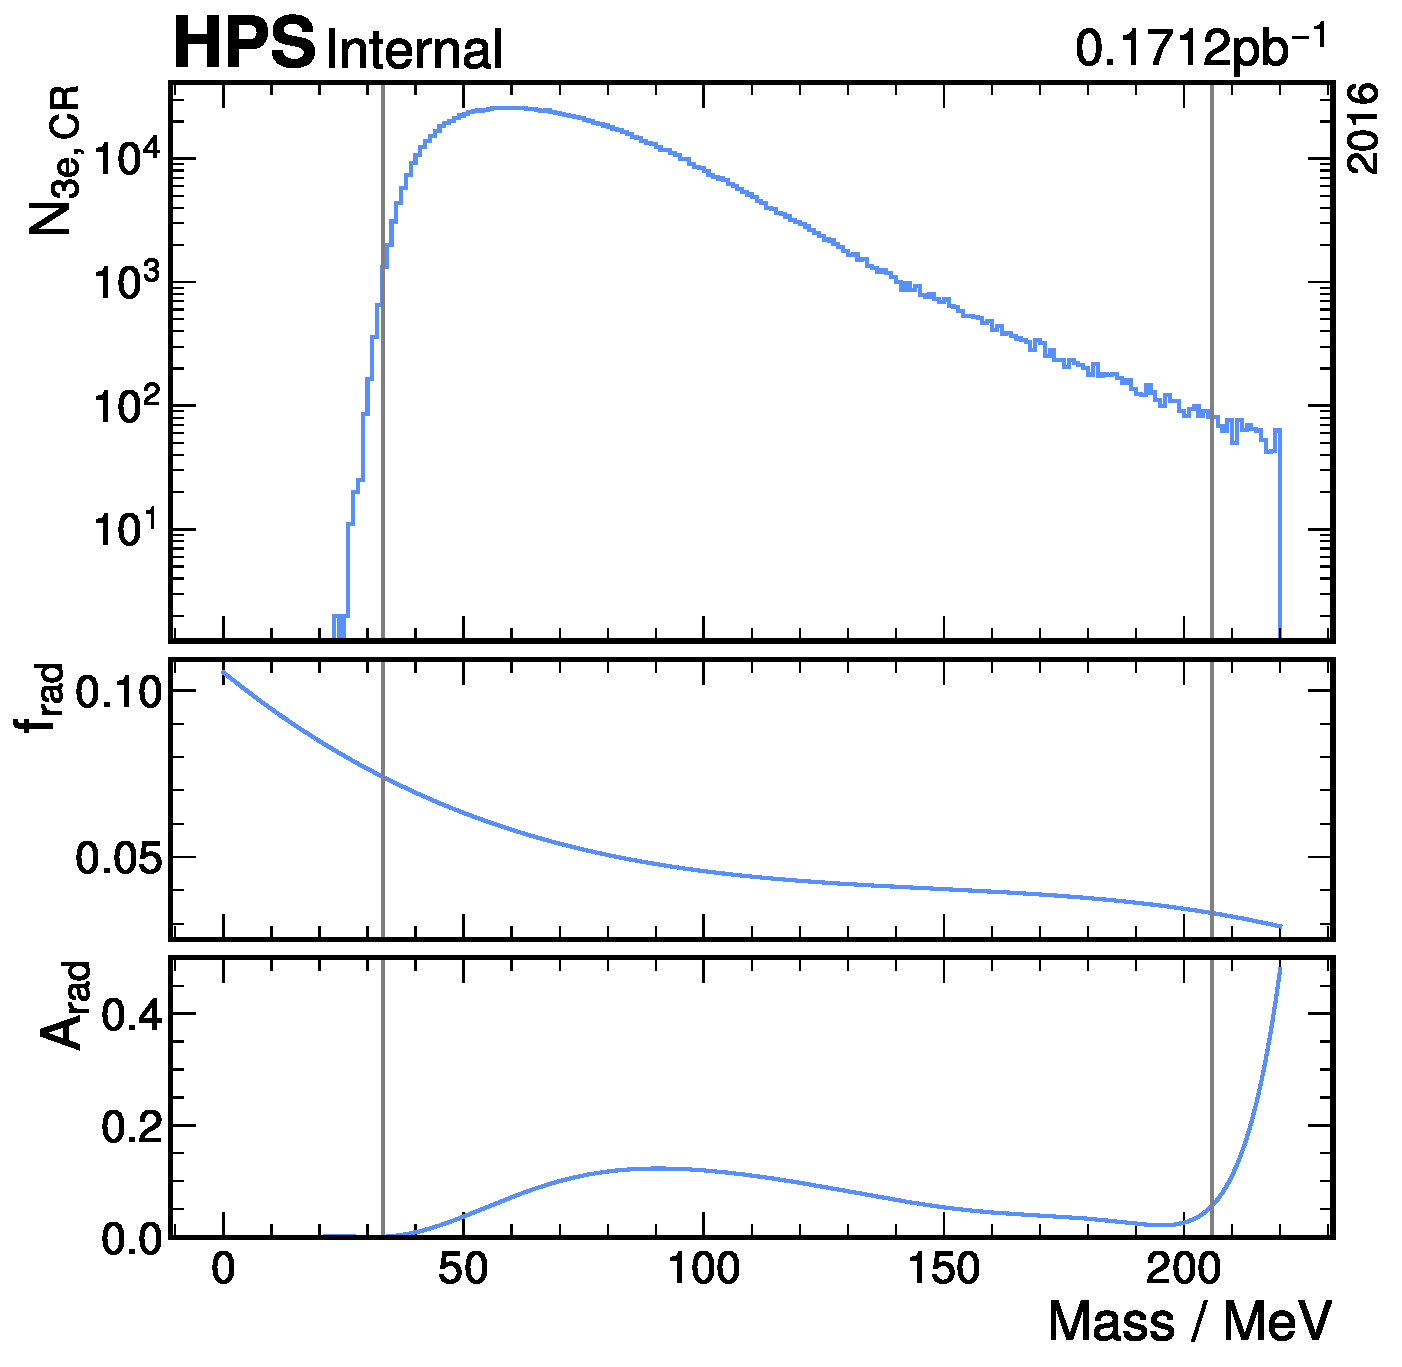
\includegraphics[width=\textwidth]{figures/hps/analysis/signal-yield/dark-photon-yield-calc-ingredients.pdf}
    \caption{Ingredients to the total dark photon yield calculation including
    the observed trident yield (top), radiative fraction (middle), and
    radiative acceptance (bottom).}
    \label{fig:dark-photon-yield-calc:ingredients}
  \end{subfigure}
  \begin{subfigure}[T]{0.48\textwidth}
    \centering
    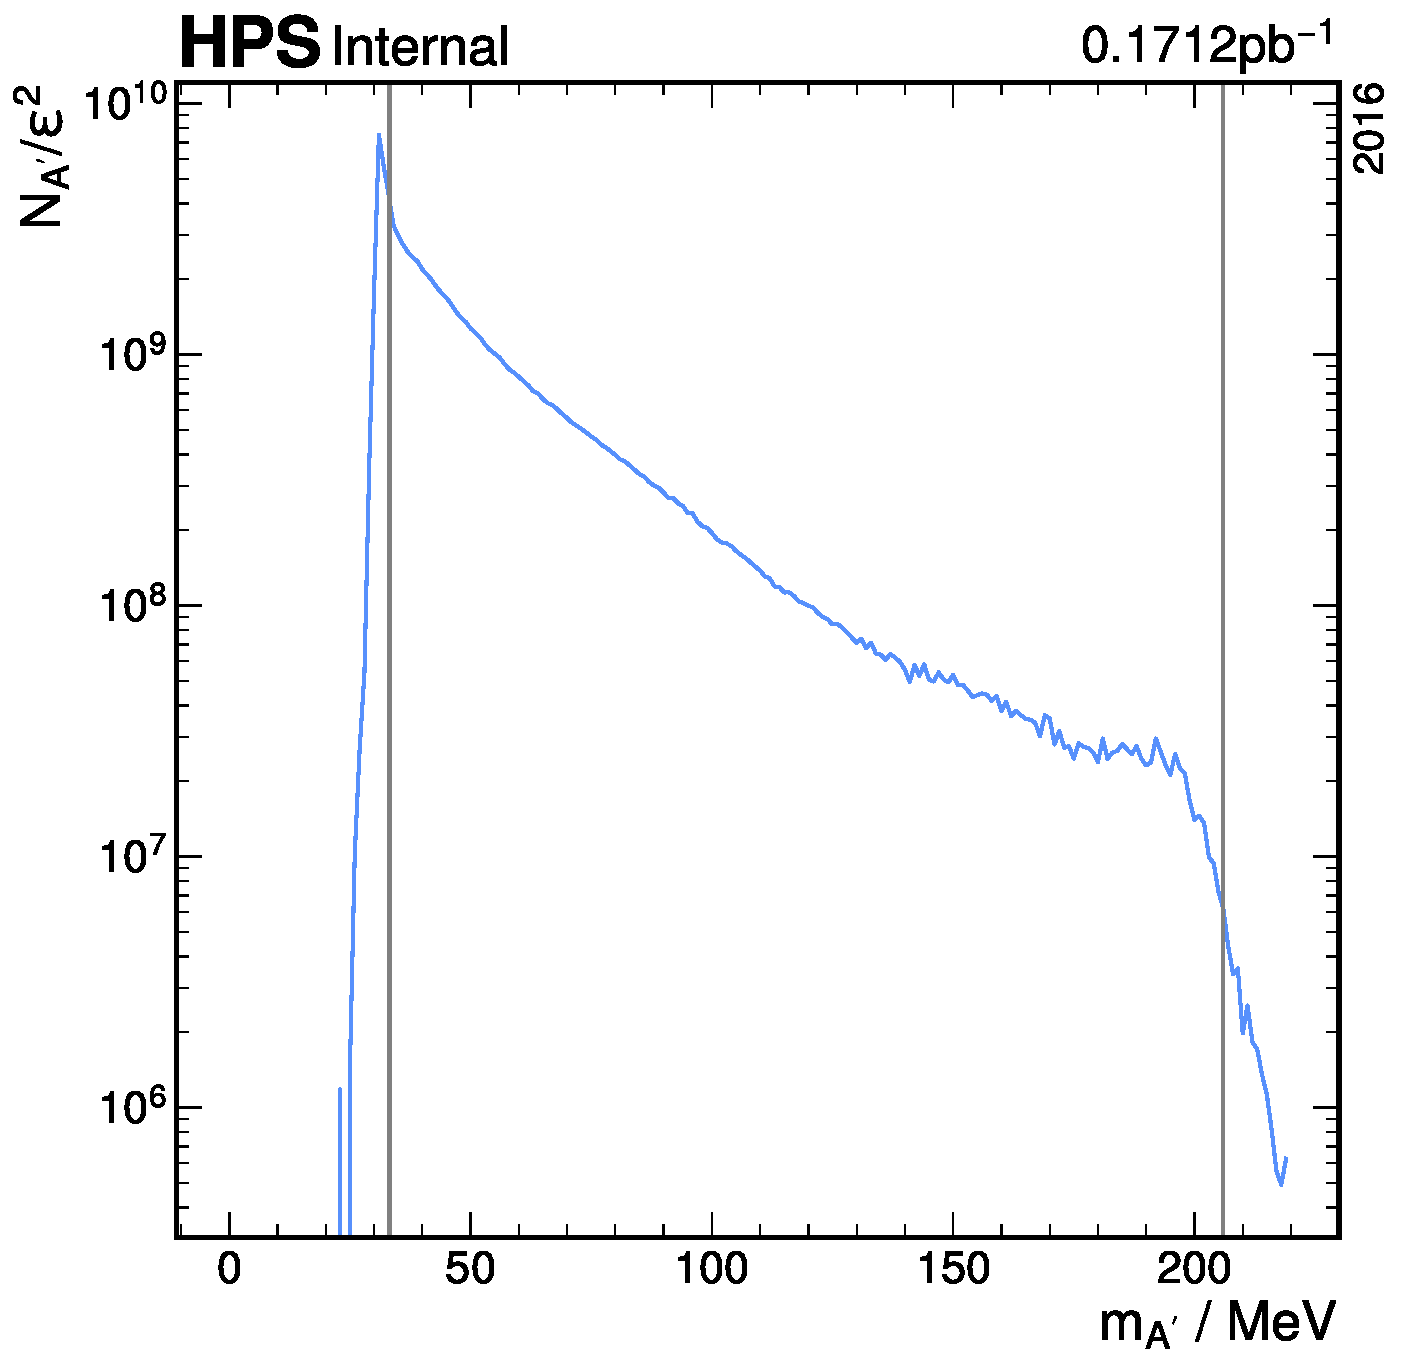
\includegraphics[width=\textwidth]{figures/hps/analysis/signal-yield/dark-photon-yield-calc-result.pdf}
    \caption{Resulting total dark photon yield.}
    \label{fig:dark-photon-yield-calc:result}
  \end{subfigure}
  \caption{Depiction of dark photon yield calculation using a single run
  of the data ($\sim\qty{1.6}{\%}$).
  The gray vertical lines show the bounds of the search using the
  nominal ratio $m_{A'}/m_{V_D} = 1.66$.}
  \label{fig:dark-photon-yield-calc}
\end{figure}

In this signal hypothesis, we do not observe the dark photon's production or decay,
instead, the dark photon decays to an unobservable dark pion and the neutral dark
vector meson $V_D$ which in turn is what decays back into a standard model electron-positron pair.
The above calculation of $N_{A'}$ accounts for the dark photon's production, but
we need to account for the dark photon's decay and the dark vector meson's decay.
The first decay has a branching ratio $BR(A'\to\pi_D V_D)$ which is complicated
by the fact that there are actually two different dark neutral vector mesons that
fit our requirements.
The second process is embedded in the decay rate of the dark vector meson to
electron-positron pairs $\Gamma(V_D\to e^+e^-)$.\footnote{
  There are other decay processes of the $V_D$!
  Namely, the so-called ``three-prong'' decay $V_D\to\pi_De^+e^-$ would
  greatly increase the potential rate at the cost of preventing the $e^+e^-$
  from reconstructing the $m_{V_D}$ mass resonance.
}
Let $E(z)$ be the signal efficiency of the analysis as a function of the $z$ where the
$V_D$ decayed into the electron-positron pair.
Then we can sum over the possible $V_D$ and estimate the fraction of $N_{A'}$
that produce a $V_D$ which decays and passes the analysis requirements.
\begin{equation}
  N_\mathrm{sig} = N_{A'}\int_{z_\mathrm{target}}^\infty \sum_{V_D} D_{V_D}(z)E(z) dz
\end{equation}
where
\begin{equation}
  D_{V_D}(z) = BR(A'\to\pi_D V_D)
  \frac{e^{-(z-z_\mathrm{target})/(\gamma c \tau_{V_D})}}{\gamma c \tau_{V_D}}
\end{equation}
The branching ratio $BR(A'\to\pi_D V_D)$ and lifetime $\tau_{V_D}$ are taken
from \cite{simp-pheno-2018} (along with the general procedure of this estimate).
What is important to remember is that the lifetime is dependent on $\epsilon^2$,
so while increasing $\epsilon^2$ increases $N_{A'}$ it also makes the lifetime shorter
and thus the $V_D$ decay ``looks'' more like standard un-displaced background.

The $V_D$ energy (and thus the relativisitic $\gamma$) used in $D_{V_D}(z)$
is only distributed over a small range (within $\mathcal{O}(\qty{100}{\MeV})$)
so we replace it with the mean $\langle\gamma\rangle$ in order to make the
calculation more practical.
Additionally, we impose an upper limit on the decay $z$ to be \qty{25}{\cm} after
the target since the efficiency of the reconstruction past $\sim\qty{20}{\cm}$ drops to zero.
\begin{equation}
  N_\mathrm{sig} = N_{A'}
    \int_{0}^{\qty{25}{\cm}} dz'
    \sum_{V_D} \mathrm{BR}(A'\to\pi_D V_D)
    \frac{e^{-z'/(\langle\gamma\rangle c \tau_{V_D})}}{\langle\gamma\rangle c \tau_{V_D}}
    E(z'+z_\mathrm{target})
\end{equation}
where $z' = z-z_\mathrm{target}$.
\cref{fig:n-sig-eg:uniform} shows $N_\mathrm{sig}$ with a uniformly perfect signal efficiency
$E(z) = 1$ to give a sense of scale, but a slightly more realistic example is using a
step-wise signal efficiency $E(z) = 0.1$ if $\qty{20}{\mm} < z < \qty{100}{\mm}$ and $0$ otherwise
\cref{fig:n-sig-eg:step}.

\begin{figure}
  \centering
  \begin{subfigure}{0.48\textwidth}
    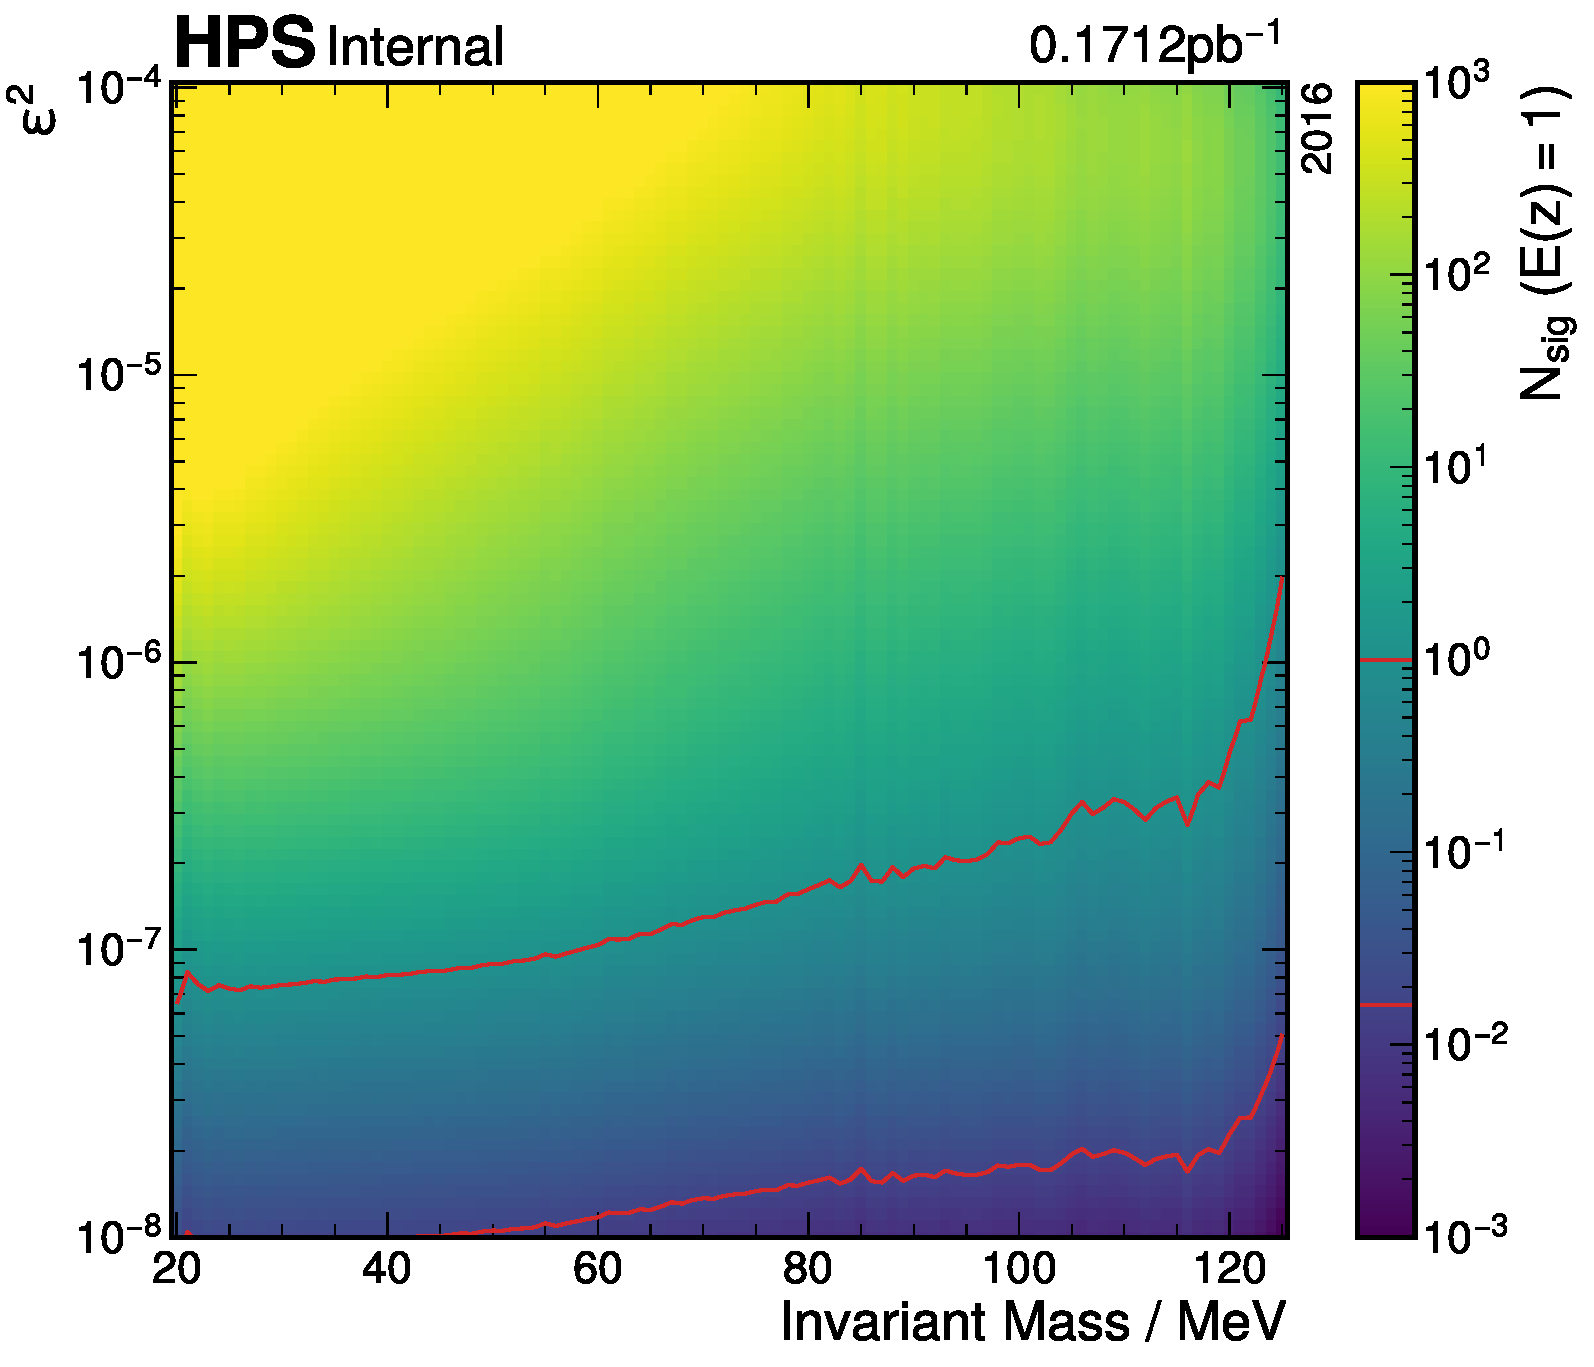
\includegraphics[width=\textwidth]{figures/hps/analysis/signal-yield/n-sig-uniform-eff-1.0.pdf}
    \caption{Uniformly perfect signal efficiency with yield dominated by prompt decays.}
    \label{fig:n-sig-eg:uniform}
  \end{subfigure}
  ~
  \begin{subfigure}{0.48\textwidth}
    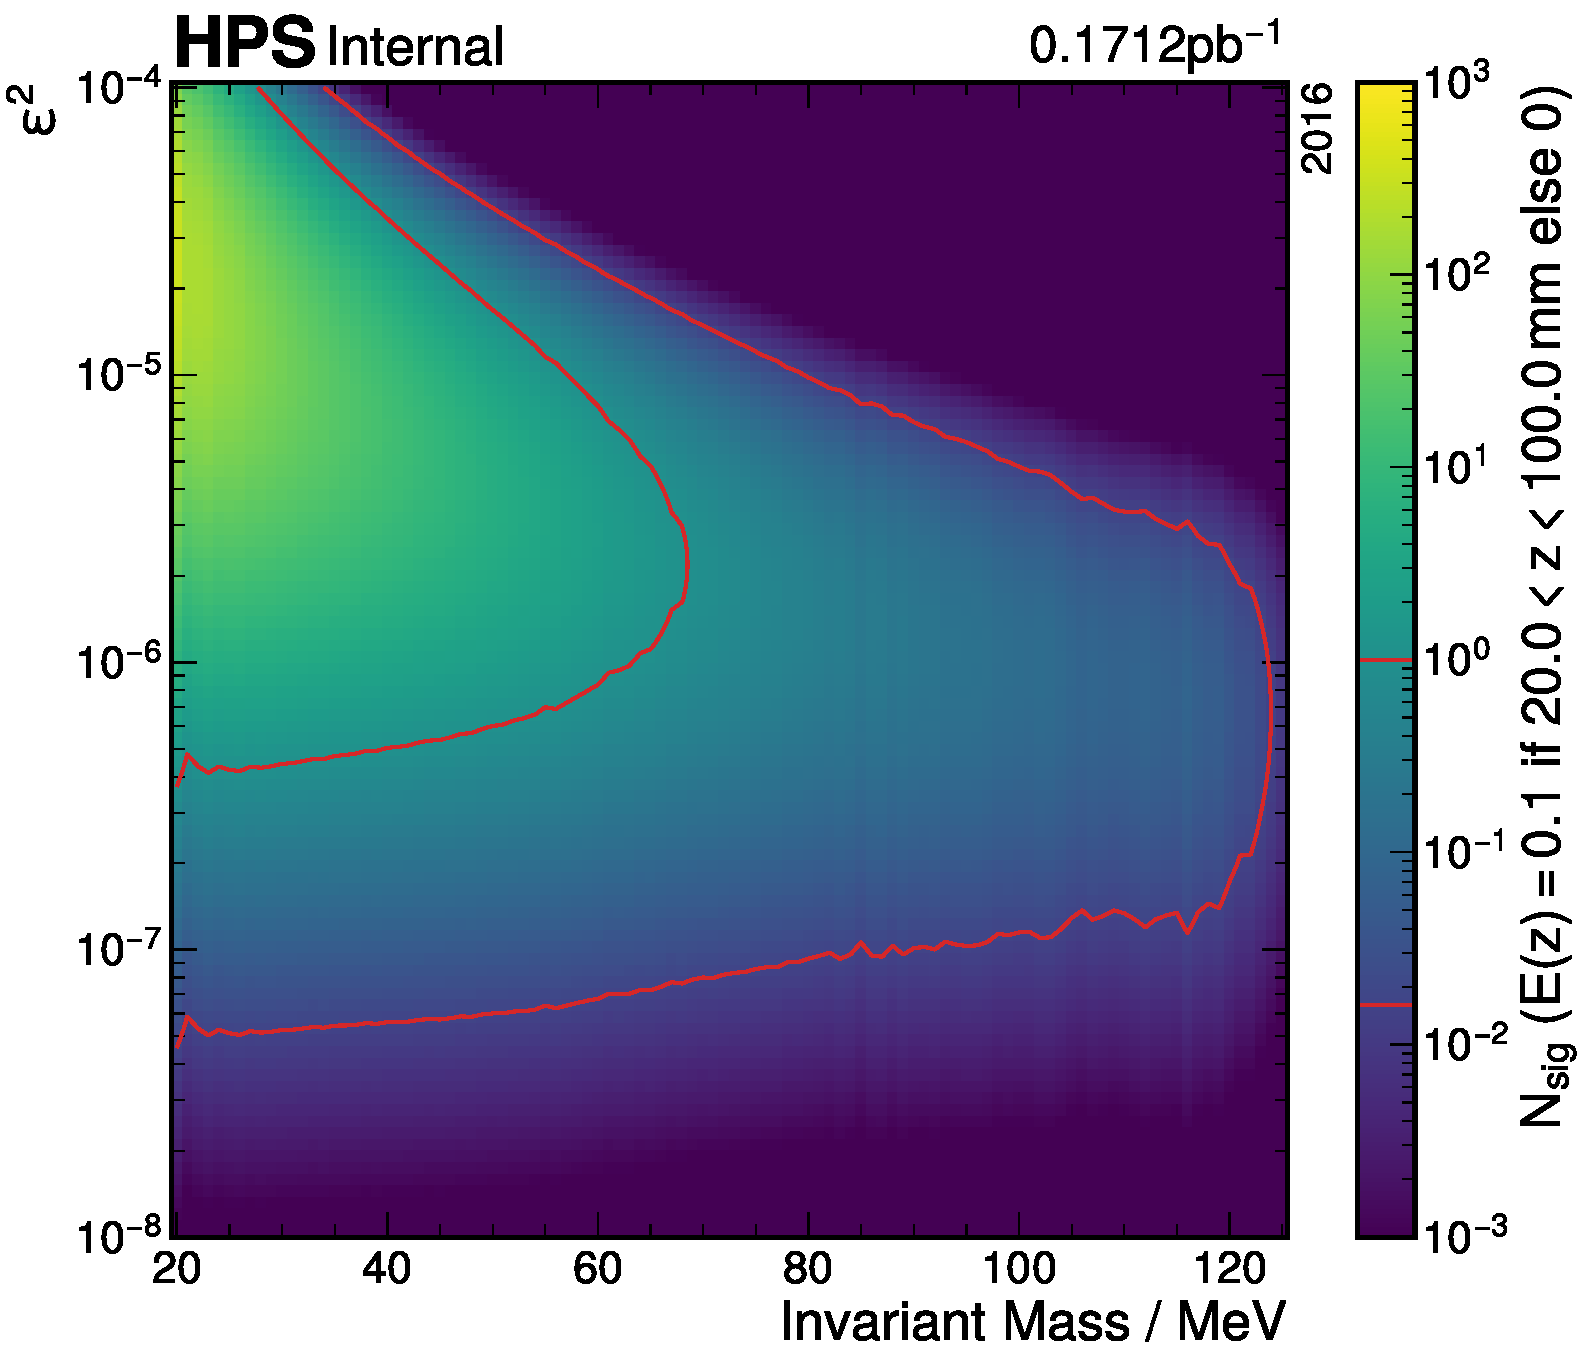
\includegraphics[width=\textwidth]{figures/hps/analysis/signal-yield/n-sig-step-eff-0.1-after-20.0.pdf}
    \caption{A step signal efficiency mocking a perfect analysis cut in displaced vertex $z$.}
    \label{fig:n-sig-eg:step}
  \end{subfigure}
  \caption{Expected signal yield $N_\mathrm{sig}$ for some rudimentary example efficiencies.
  Red contour lines are given at 1 and 1.6\% (the approximate fraction of this data subsample)
  to give a sense of scale.
  Values are ``clipped'' to the color bar (for example, a signal yield of \num{2e4} is colored
  yellow which is marked as \num{1e3}) so we can focus on the important orders of magnitude.}
  \label{fig:n-sig-eg}
\end{figure}

In summary, the key point to make here is that the signal efficiency as a function of true
decay length $E(z)$ is the single analysis-dependent ingredient that effects the resulting
signal yield.
The rest of the ingredients are either fixed by the dataset being searched (e.g. trident
differential production, $f_\mathrm{rad}$, $A_\mathrm{rad}$) or are parameters that we
vary for the search ($\epsilon^2$, $m_{V_D}$).
A moderately realistic signal efficiency shows the range of $\epsilon^2$ and $m_{V_D}$
in which this dataset has potential sensitivity (\cref{fig:n-sig-eg:step}) which informs the
ranges these values will take below.


\section{Reconstruction Categories}
\label{sec:hps:recon-cat}
The design of \ac{hps} separates reconstructed tracks into categories that are
not necessarily associated with the underlying physics for which we are searching.
Specifically, the number of layers (and which layers) that are included within a track
has a large effect on the resulting precision of the reconstructed physics variables
of that track; thus, we categorize vertices on whether one or both of their tracks contain
both sensors in the first layer.
\cref{fig:hps-reco-category-diagram} shows examples of the two categories considered
within this work.
The L1L1 category whose verticies have both tracks with good precision was first studied
for this signal search\cite{aspellman-thesis-2024} when optimizing the pre-selection
requirements described earlier.

Extending this search to the L1L2 category has a rather simple motivation.
While the vertices may degrade in precision, the additional increase of data both in terms
of total volume and the potential to observe higher-displaced vertices is expected to improve
the sensitivity of the \ac{hps} \ac{simp} search.

\begin{figure}
  \centering
  \begin{subfigure}{0.48\textwidth}
    \centering
    \resizebox{\textwidth}{!}{\begin{tikzpicture}
  \drawhpsfirsttwolayers
  \node at (\targetx,+2) {L1L1};
  \node at (\targetx+1,0.1) [circle,fill,inner sep=1.5pt] {};
  \draw[black,->] (\targetx+1,0.1) -- (2.5,2) node[anchor=north west] {\(e^-\)};
  \draw[black,->] (\targetx+1,0.1) -- (2.5,-1.9) node[anchor=south west] {\(e^+\)};
\end{tikzpicture}
}
  \end{subfigure}
  ~
  \begin{subfigure}{0.48\textwidth}
    \centering
    \resizebox{\textwidth}{!}{\begin{tikzpicture}
  \drawhpsfirsttwolayers
  \node at (\targetx,+2) {L1L2};
  \node at (\targetx+2.0,0.1) [circle,fill,inner sep=1.5pt] {};
  \draw[black,->] (\targetx+2.0,0.1) -- (2.5,2) node[anchor=north west] {\(e^-\)};
  \draw[black,->] (\targetx+2.0,0.1) -- (2.5,-1.8) node[anchor=south west] {\(e^+\)};
\end{tikzpicture}
}
  \end{subfigure}
  \caption{Diagrams showing L1L1 (left) and L1L2 (right) vertex examples.}
  \label{fig:hps-reco-category-diagram}
\end{figure}

\section{Physics Variables}
\label{sec:hps:analysis:variables}
There are many possible variables that could be used to separate candidate signal
vertices from the standard process backgrounds.
While this section is not an exhaustive list of all possible variables,
it does explain the ones used within this analysis as well as motivation for
their use.

The \ac{simp} signal vertex will have significantly less energy than the amount
delivered by the beam because of the production of a light dark meson when the heavier
vector meson $V_D$ is produced.
Thus, a selection on the sum of the momentum magnitudes is applied.
\begin{equation}
  P_\mathrm{sum} = |\vec{p}_{e^-}|+|\vec{p}_{e^+}|
\end{equation}
Specifically, the Signal Region (SR) used for the actual search requires
$\qty{1.0}{\GeV} < $\Psum$ < \qty{1.9}{\GeV}$ and the Control Region (CR)
used for determining the trident differential production rate is
$\qty{1.9}{\GeV} < $\Psum$ < \qty{2.4}{\GeV}$.

Since we are searching for the dark vector boson $V_D$ via its
2-body decay into an electron and a positron, we expect the invariant mass of the vertex $m_\text{reco}$
to be within the resolution of the detector $\sigma_m$ of the mass we are searching for $m_{V_D}$.
\begin{equation}
  p_m = \frac{|m_\text{reco}-m_{V_D}|}{\sigma_m}
\end{equation}
Applying an upper limit on $p_m$ is often refered to as a ``mass window''
since it results in $m_\text{reco}$ residing within a small range around $m_{V_D}$.
For optimizing the other selections, $p_m < 2.8$ is used.
The search for a potential excess of \ac{simp}-like events is using sidebands
along $m_\mathrm{reco}$ in data so no selection on $p_m$ is imposed when searching.
The estimate of the resulting sensitivity uses the signal region selection from
the search of $p_m < 1.5$.

Each vertex can be projected back to the target using its position and total momentum,
and the location of the vertex at the target can be compared to the beam
position extracted from 1\% of each data-collection run.
The separation between the projected position $\vec{x} = (x,y)$ and the beam position
$\vec{\mu} = (\mu_{x'}, \mu_{y'})$ is then measured
and normalized by the width of the beam in that direction $(\sigma_{x'},\sigma_{y'})$.
The distribution of the beamspot is allowed to be rotated relative to our
chosen axes by the angle $\theta_\mathrm{beam}$, meaning we need to rotate $\vec{x}$
before comparing it to the beam spot.
The total ``elliptical'' separation between the reconstructed vertex
projected back to the target and the beam spot can be quantified by
\begin{equation}
  N_\sigma = \sqrt{
    \left(
      \frac{x\cos\theta_\mathrm{beam} - y\sin\theta_\mathrm{beam} - \mu_{x'}}{\sigma_{x'}}
    \right)^2
    +\left(
      \frac{x\sin\theta_\mathrm{beam} + y\cos\theta_\mathrm{beam} - \mu_{y'}}{\sigma_{y'}}
    \right)^2
  }
\end{equation}
I refer to this as \ac{vps} since it represents how significantly
a vertex deviates from originating at the beam spot.
% maybe comment on how an upper limit on this variable is useful?

Since the detector's tracking modules are oriented to be most senstive in the
vertical direction, the vertical impact parameter $y_0$ has higher precision compared
to the horizontal impact parameter.
For truly-displaced signal vertices, both tracks making the vertex would have
$y_0$ far from zero while background vertices would have at least one track
with $y_0$ near zero (undisplaced vertices would have both, but mis-reconstructed
fake-displaced vertices could have one far from zero).
\cref{fig:hps-displace-eg} shows some diagrams that illuminate this effect.
While there are many ways for a vertex to end up being ``fake displaced''
(for example, a missing or mis-chosen hit in the first layer like the example shown
in \cref{fig:hps-displace-eg}), forcing both $y_0$ to be far from zero removes
these background processes.
This motivates selecting vertices based on requiring the minimum of the two
absolute value $y_0$ to be above a certain threshold.
\begin{equation}
  y_{0,\min} = \min(|y_{0,e^-}|,|y_{0,e^+}|)
\end{equation}
which more sharply distinguishes truly displaced vertices compared to the
vertex $z$ often muddled by fake-displaced vertices where one track is
mis-reconstructed at high $|y_0|$.

\begin{figure}
  \begin{subfigure}{0.32\textwidth}
    \resizebox{\textwidth}{!}{\begin{tikzpicture}
  \drawhpsfirsttwolayers
  \draw[black] (\targetx-\targethalfthick,0) -- (2.5,0);
  \node[anchor=north west,align=left,text depth=\baselineskip] at (\targetx,+3)
    {Truly\\Displaced};
  \node at (\targetx+2,0.1) [vertex] {};
  \draw[black,->] (\targetx+2.0,0.1) -- (2.5,2) node[anchor=north west] {\(e^-\)};
  \node at (\layeronex-\sensorhalfsep,\elelayeronestereoy) [hit] {};
  \node at (\layeronex+\sensorhalfsep,\elelayeroneaxialy) [hit] {};
  \node at (\layertwox-\sensorhalfsep,\elelayertwostereoy) [hit] {};
  \node at (\layertwox+\sensorhalfsep,\elelayertwoaxialy) [hit] {};
  \draw[black,->] (\targetx+2.0,0.1) -- (2.5,-1.8) node[anchor=south west] {\(e^+\)};
  \node at (\layeronex-\sensorhalfsep,\poslayeronestereoy) [miss] {};
  \node at (\layeronex+\sensorhalfsep,\poslayeroneaxialy) [miss] {};
  \node at (\layertwox-\sensorhalfsep,\poslayertwostereoy) [hit] {};
  \node at (\layertwox+\sensorhalfsep,\poslayertwoaxialy) [hit] {};
  \draw[black,dotted]
    (\targetx+2,0.1) -- (\targetx,\eleyzero)
    (\targetx+2,0.1) -- (\targetx,\posyzero);
  \draw[decoration={brace,raise=5pt},decorate]
    (\targetx,\eleyzero) -- node[left=6pt] {$y_{0}^{e^-}$} (\targetx,0);
  \draw[decoration={brace,raise=5pt},decorate]
    (\targetx,0) -- node[left=6pt] {$y_{0}^{e^+}$} (\targetx,\posyzero);
\end{tikzpicture}
}
  \end{subfigure}
  \begin{subfigure}{0.32\textwidth}
    \resizebox{\textwidth}{!}{\begin{tikzpicture}
  \drawhpsfirsttwolayers
  \draw[black] (\targetx-\targethalfthick,0) -- (2.5,0);
  \node[anchor=north west,align=left] at (\targetx,+3)
    {Fake Displaced\\$y_0^{e^-}\approx\qty{0}{\mm}$};

  \draw[black,->] (\targetx+\targethalfthick,0.0) -- (2.5,2) node[anchor=north west] {\(e^-\)};
  \node at (\layeronex-\sensorhalfsep,\fdelelayeronestereoy) [hit] {};
  \node at (\layeronex+\sensorhalfsep,\fdelelayeroneaxialy) [hit] {};
  \node at (\layertwox-\sensorhalfsep,\fdelelayertwostereoy) [hit] {};
  \node at (\layertwox+\sensorhalfsep,\fdelelayertwoaxialy) [hit] {};

  \draw[black,->] (\fdposx, \fdposy) -- (2.5,-1.8) node[anchor=south west] {\(e^+\)};
  \draw[dashed] (\layertwox,\fdposlayertwoaxialy) -- (\targetx+\targethalfthick,0.0)
    node[near start,below,sloped,font=\scriptsize] {True \(e^+\)};
  \node at (\layeronex-\sensorhalfsep,\fdbadhitstereoy) [hit] {};
  \node at (\layeronex+\sensorhalfsep,\fdbadhitaxialy) [miss] {};
  \node at (\layeronex-\sensorhalfsep,\fdtruhitstereoy) [miss] {};
  \node at (\layeronex+\sensorhalfsep,\fdtruhitaxialy) [miss] {};
  \node at (\layertwox-\sensorhalfsep,\fdposlayertwostereoy) [hit] {};
  \node at (\layertwox+\sensorhalfsep,\fdposlayertwoaxialy) [hit] {};

  \node at (\fdposx,\fdposy) [vertex] {};

  \draw[black,dotted] (\fdposx,\fdposy) -- (\targetx,\fdposyzero);

  \draw[decoration={brace,raise=5pt},decorate]
    (\targetx,0) -- node[left=6pt] {$y_{0}^{e^+}$} (\targetx,\fdposyzero);

%  \node[vertex,label=right:{Vertex}] (vtxlabel) at (\targetx,-2.0) {};
%  \node[hit,label=right:{Hit},below=5.0pt of vtxlabel] (hitlabel) {};
%  \node[miss,label=right:{Missed},below=5.0pt of hitlabel] {};

%  \node[vertex,label=right:{Vertex}] (vtxlabel) at (\targetx,+3.0) {};
%  \node[hit,label=right:{Hit}] at (\targetx+1.8,+3.0) {};
%  \node[miss,label=right:{Missed}] at (\targetx+3.0,+3.0) {};
\end{tikzpicture}
}
  \end{subfigure}
  \begin{subfigure}{0.32\textwidth}
    \resizebox{\textwidth}{!}{\begin{tikzpicture}
  \drawhpsfirsttwolayers
  \draw[black] (\targetx-\targethalfthick,0) -- (2.5,0);

  \node[align=left] at (\targetx,+2) {Not Displaced\\$y_0^{e^-}\approx\qty{0}{\mm}$\\$y_0^{e^+}\approx\qty{0}{\mm}$};
  \draw[black,->] (\targetx+\targethalfthick,0.0) -- (2.5,2) node[anchor=north west] {\(e^-\)};
  \draw[black,->] (\targetx+\targethalfthick,0.0) -- (2.5,-1.8) node[anchor=south west] {\(e^+\)};
  \node at (\targetx+\targethalfthick,0.0) [circle,fill,inner sep=1.5pt] {};
\end{tikzpicture}
}
  \end{subfigure}
  \caption{Diagrams of examples for how different types of L1L2 vertices effect the observed
  values of $y_0$.
  Truly displaced vertices (left) have both tracks whose $y_0$ is far
  from $\qty{0}{\mm}$ while fake displaced vertices (middle) and not displaced (right)
  have at least one if not both tracks with $y_0\approx\qty{0}{\mm}$.
  The diamonds are the reconstructed vertex, the solid circles are the reconstructed hits,
  and the empty circles are ``missed'' hits.}
  \label{fig:hps-displace-eg}
\end{figure}

The track fit uncertainty of the vertical impact parameter $\sigma_{y_0}$
is a helpful quality parameter measuring how confident the track fit is
in the $y_0$ value.
Placing an upper limit on this value for both tracks within a vertex
effectively requires both tracks to have good vertical resolution,
helping remove some highly-displaced vertices presumably arising
from mis-reconstructed tracks.
\begin{equation}
  \sigma_{y_0,\max} = \max(\sigma_{y_0,e^-},\sigma_{y_0,e^+})
\end{equation}

\cref{fig:data-signal-comp} displays the distributions of these last three
variables for a few example mass points after the other, solidified selections
(L1L2 vertex, the momentum sum is in the Signal Region, and the invariant mass
falls within the chosen mass window).

\begin{figure}
  \centering
  \begin{subfigure}{0.30\textwidth}
    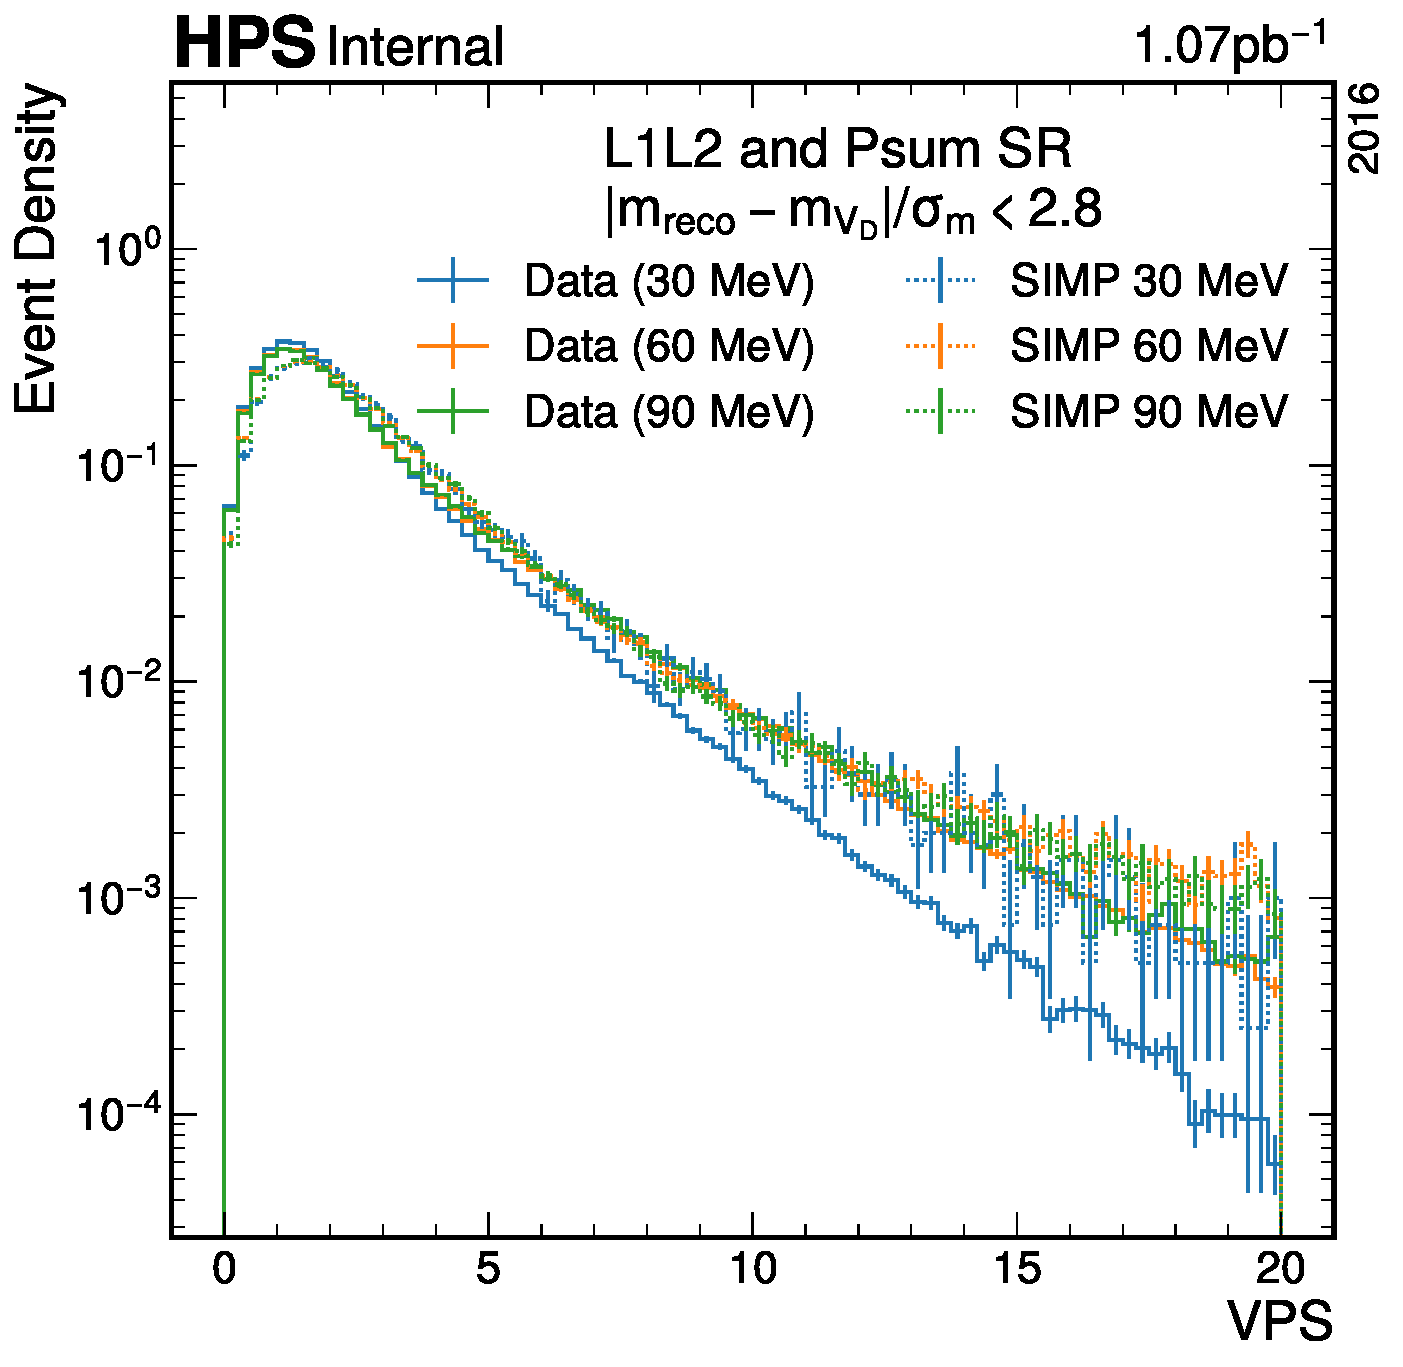
\includegraphics[width=\textwidth]{figures/hps/analysis/vtx_proj_sig-distribution.pdf}
    \caption{\ac{vps}}
    \label{fig:data-signal-comp:vps}
  \end{subfigure}
  ~
  \begin{subfigure}{0.30\textwidth}
    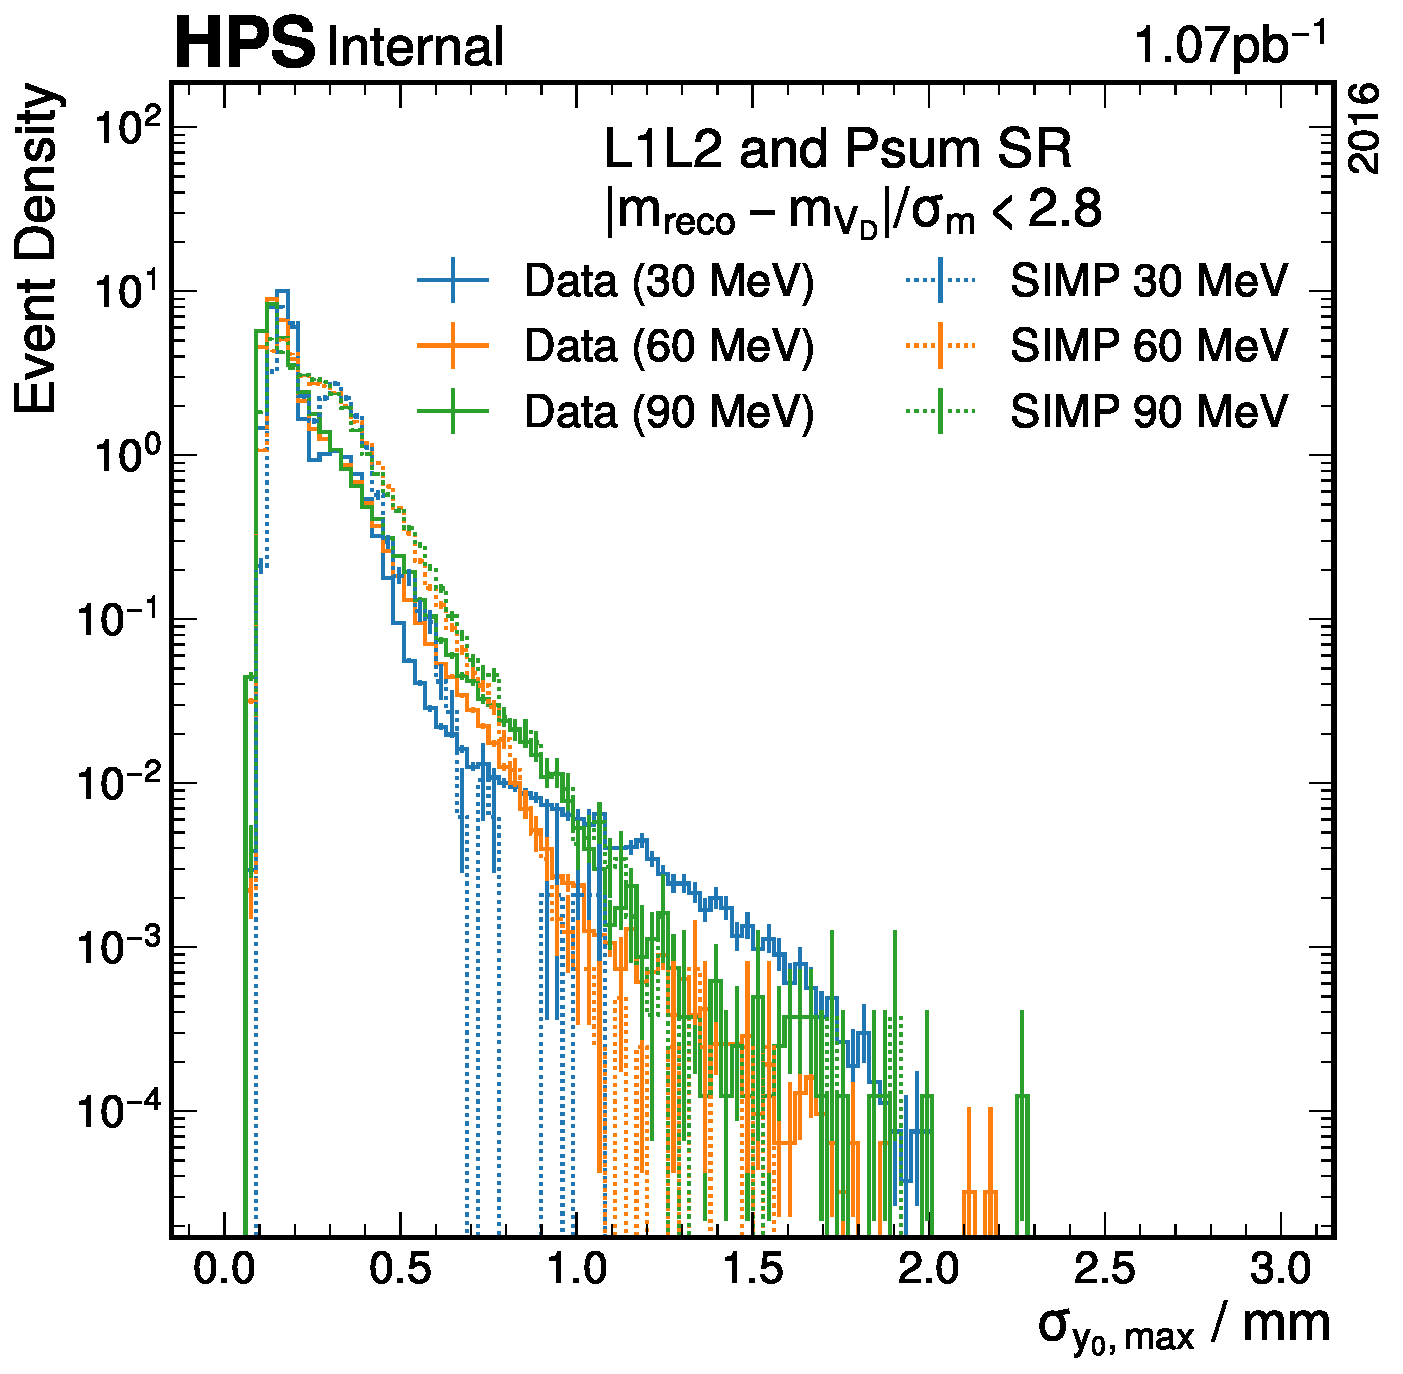
\includegraphics[width=\textwidth]{figures/hps/analysis/max_y0_err-distribution.pdf}
    \caption{\maxyzeroerr}
    \label{fig:data-signal-comp:max-y0-err}
  \end{subfigure}
  ~
  \begin{subfigure}{0.30\textwidth}
    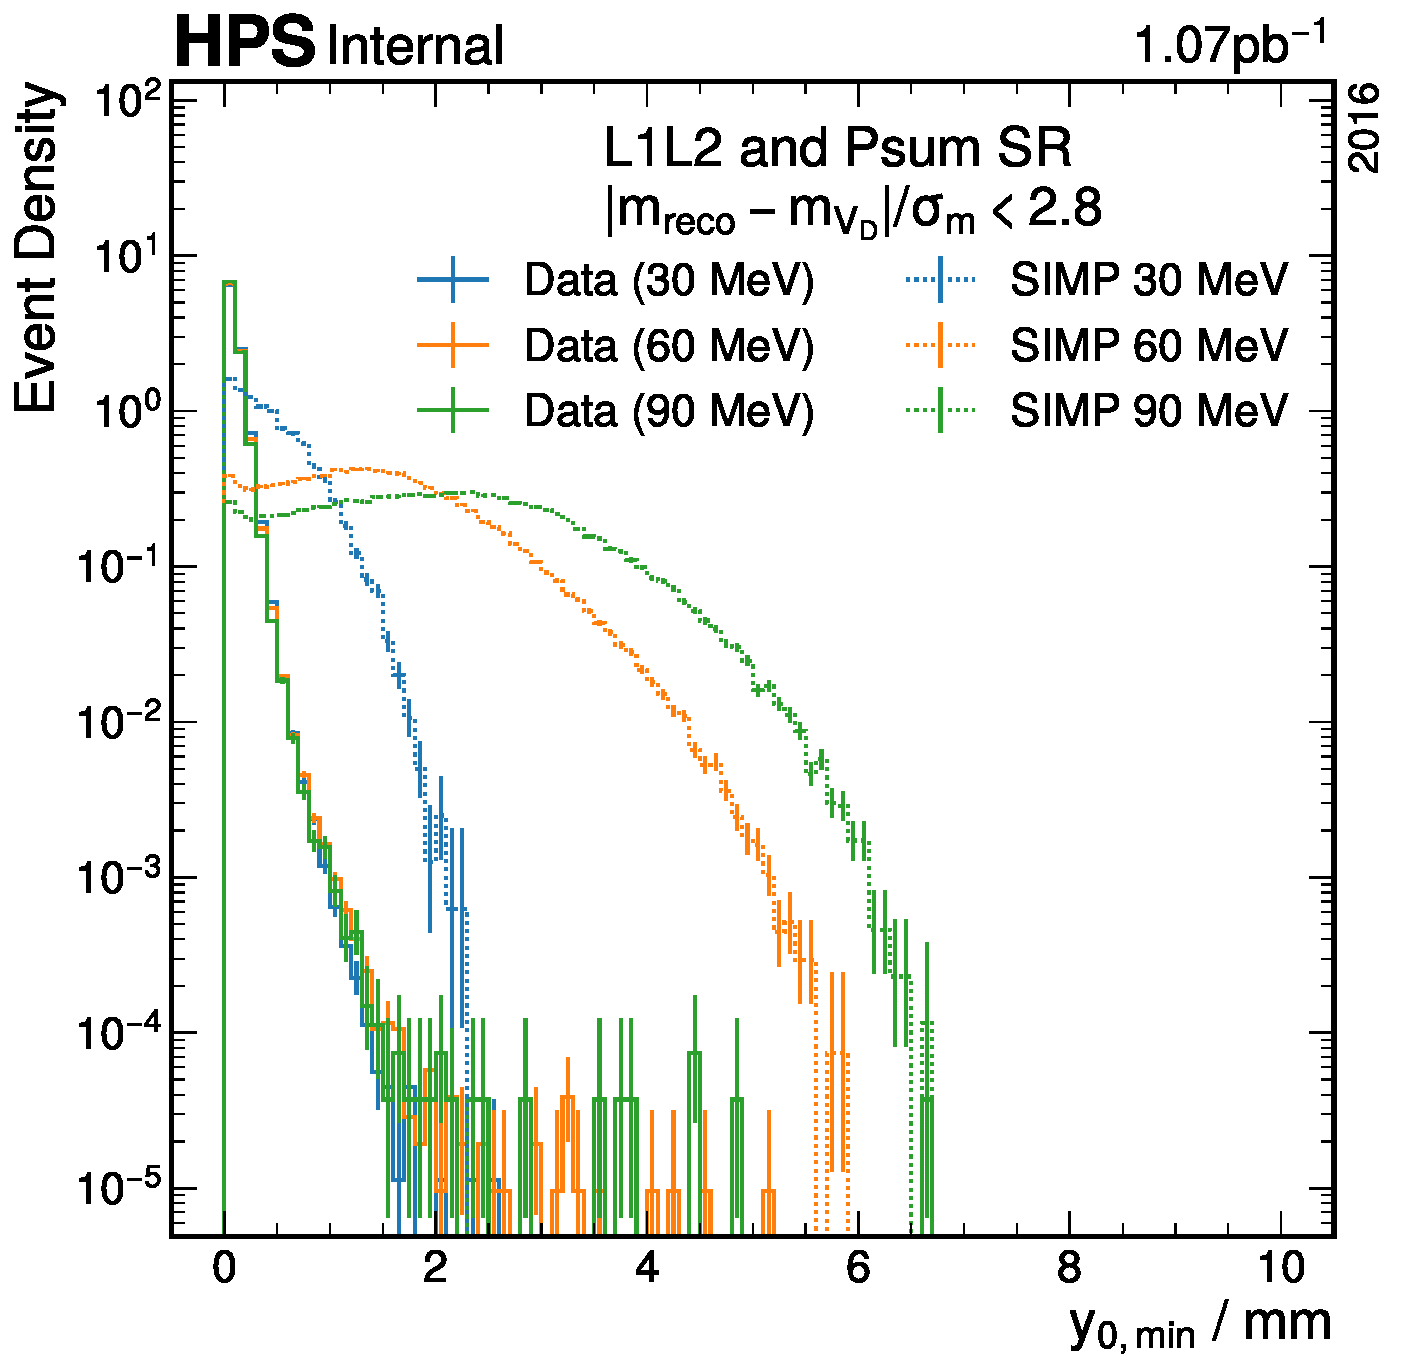
\includegraphics[width=\textwidth]{figures/hps/analysis/min_y0-distribution.pdf}
    \caption{\minyzero}
    \label{fig:data-signal-comp:min-y0}
  \end{subfigure}
  \caption{%
    Distributions of cut variables for a few example mass points and $\approx10\%$ of the full data sample.
    The vertices are required to be L1L2, have their momentum sum be within
    the signal region, and their invariant mass within the specified mass window.
  }
  \label{fig:data-signal-comp}
\end{figure}

Vertex $z$ is left for late-stage statistical analysis of the results
and -- being highly correlated with \minyzero -- is redundant with this variable.

\section{Selection}
The selection on these variables was optimized using a subsample of the collected
data amounting to $\approx10\%$ of the full sample.
All of the variables except the last, separating variable (\minyzero) were varied
while keeping the relative signal efficiency high ($>\qty{80}{\%}$), focused on
removing the highly-displaced events leading to the long tail in data observed
in \cref{fig:data-signal-comp:min-y0}.
\cref{fig:min-y0-after-others} shows the cleaned \minyzero distribution after
these selections.
There are still a few highly-displaced events left; however, removing them
incurs a higher penalty on signal efficiency and leads to a lower resulting
sensitivity estimated from this subsample.

\begin{figure}
  \centering
  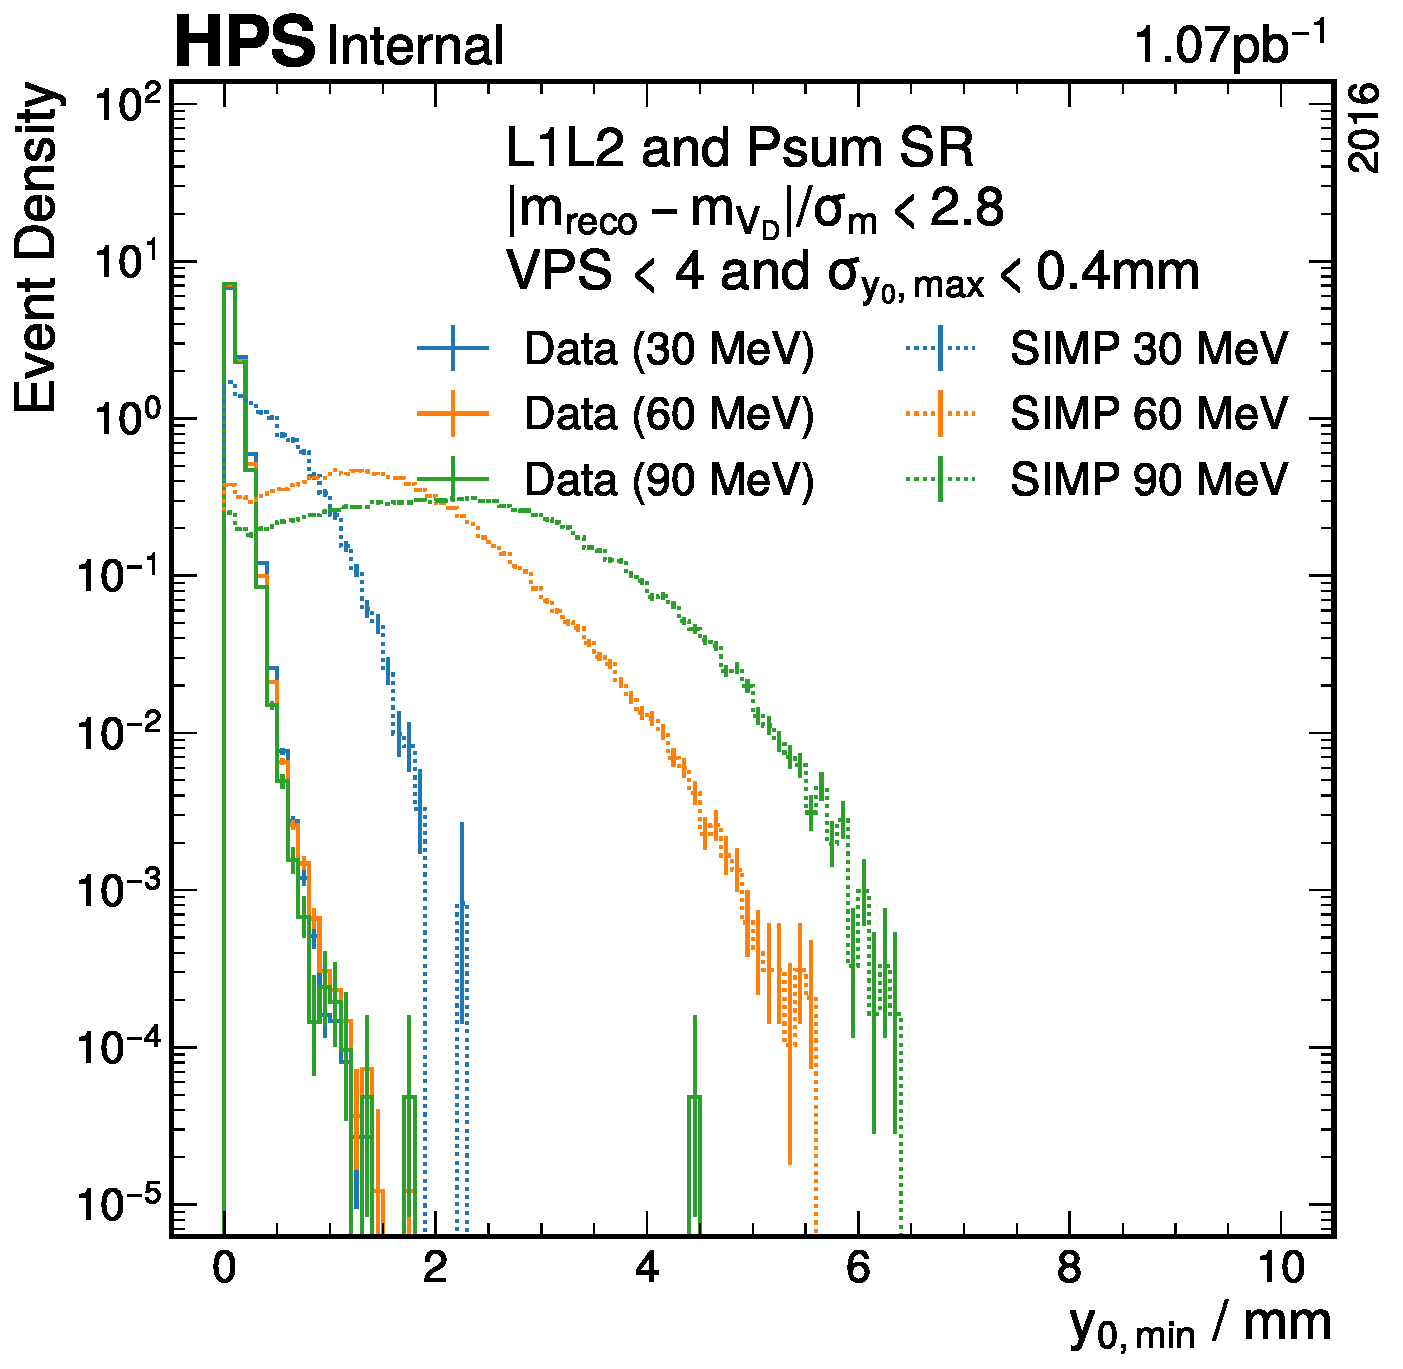
\includegraphics[width=0.5\textwidth]{figures/hps/analysis/min-y0-after-others.pdf}
  \caption subsample.
For this optimization, the expected signal was artificially scaled such that it would
be on the same order-of-magnitude as the observed data (specifically, a scaling factor
of $0.1/\epsilon$ was found to work well although variations in this scaling factor did not vary
the chosen selections by much).

The \minyzero values chosen by this maximization (\cref{fig:miny0-opt}) are ragged due to the finite
nature of the subsample on which they are being chosen.
In order to avoid over-biasing the selection to this arbitrarily-chosen subsample,
the actual cuts used in the final analysis are smoothed by fitting a line to the area
whose maximumim binomial significance is above zero and then continuining this line with flat
values outside this region.

\begin{figure}
  \centering
  \begin{subfigure}{0.48\textwidth}
    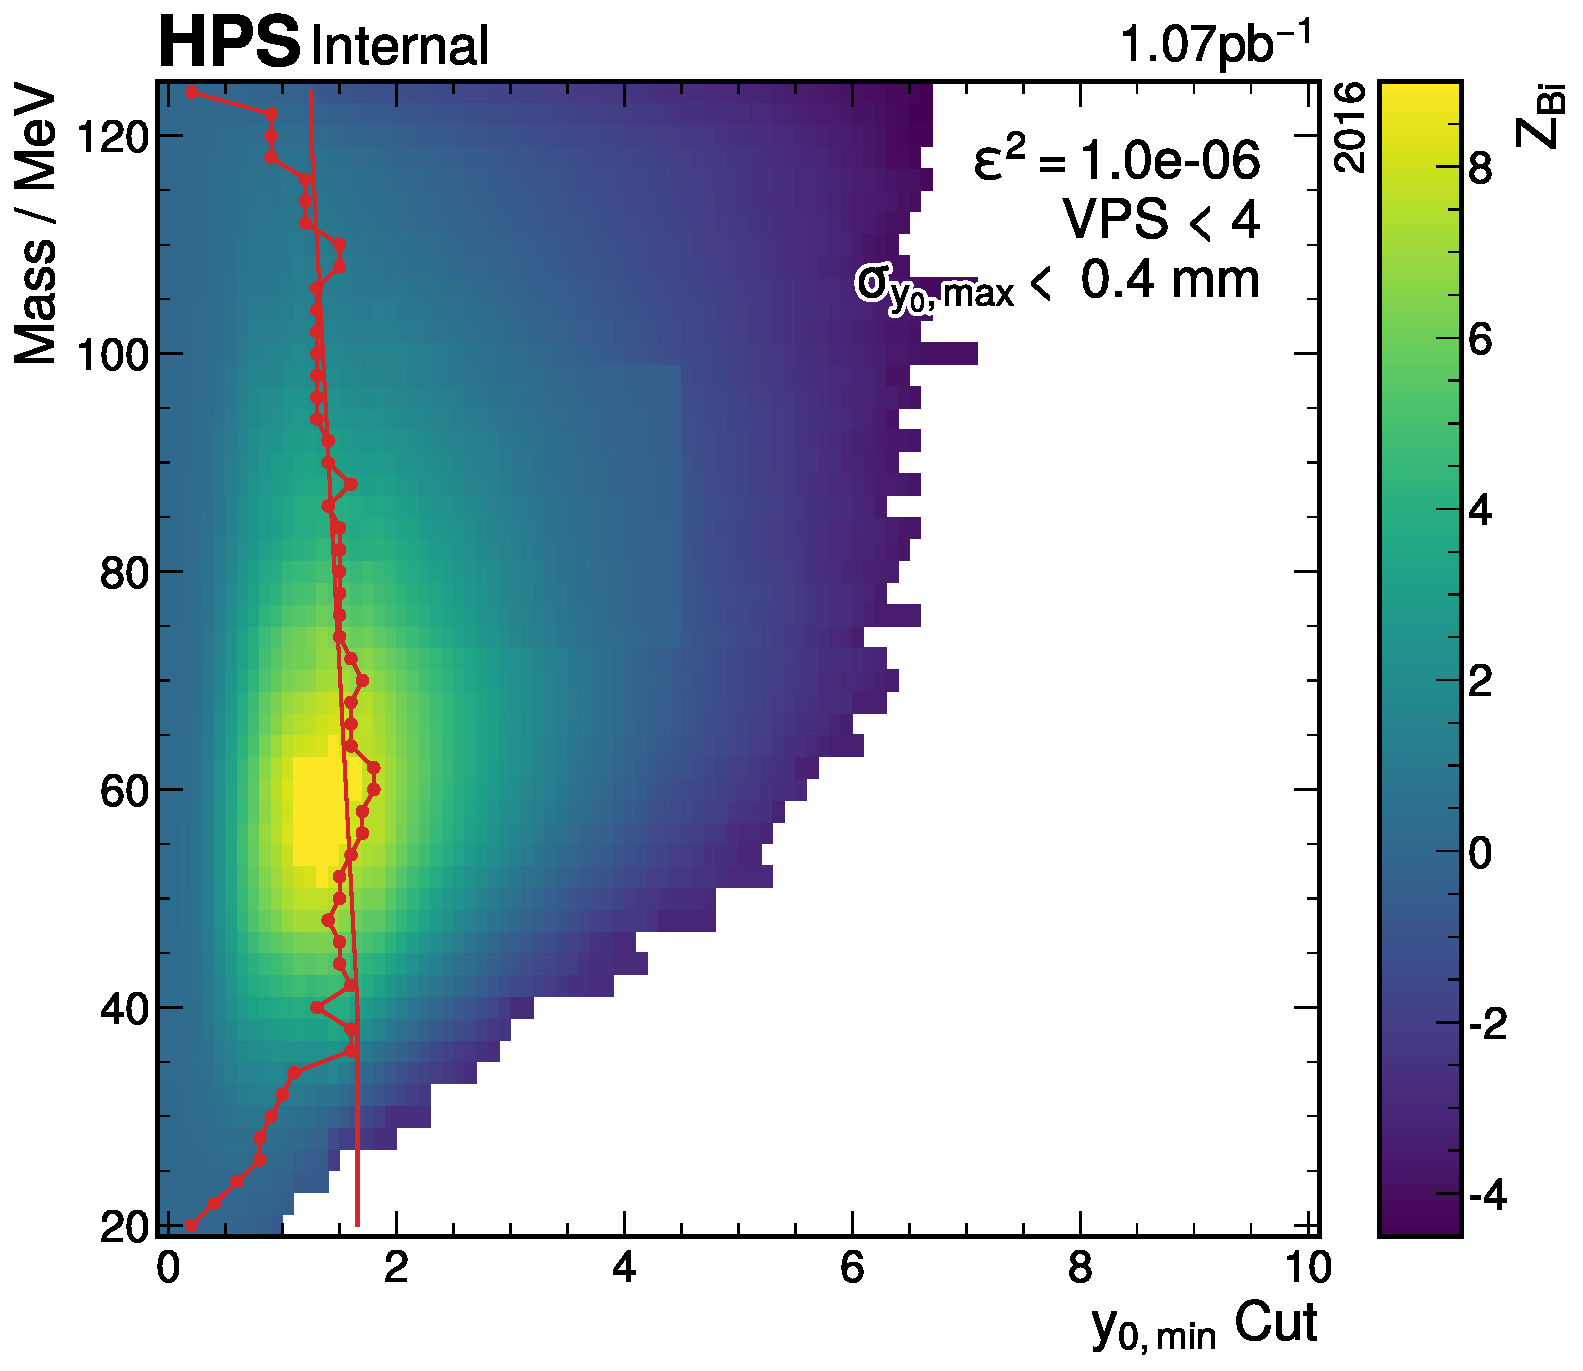
\includegraphics[width=\textwidth]{figures/hps/analysis/miny0-after-others-zbi-eps2-1e-6.pdf}
    \caption{%
      Binomial significance ($Z_\mathrm{Bi}$) for a range of masses and \minyzero cut choices
      with the points maximizing $Z_\mathrm{Bi}$ for each mass drawn in red circles and the linear fit with
      its flat continuation as a red line.
    }
    \label{fig:miny0-opt:zbi}
  \end{subfigure}
  ~
  \begin{subfigure}{0.48\textwidth}
    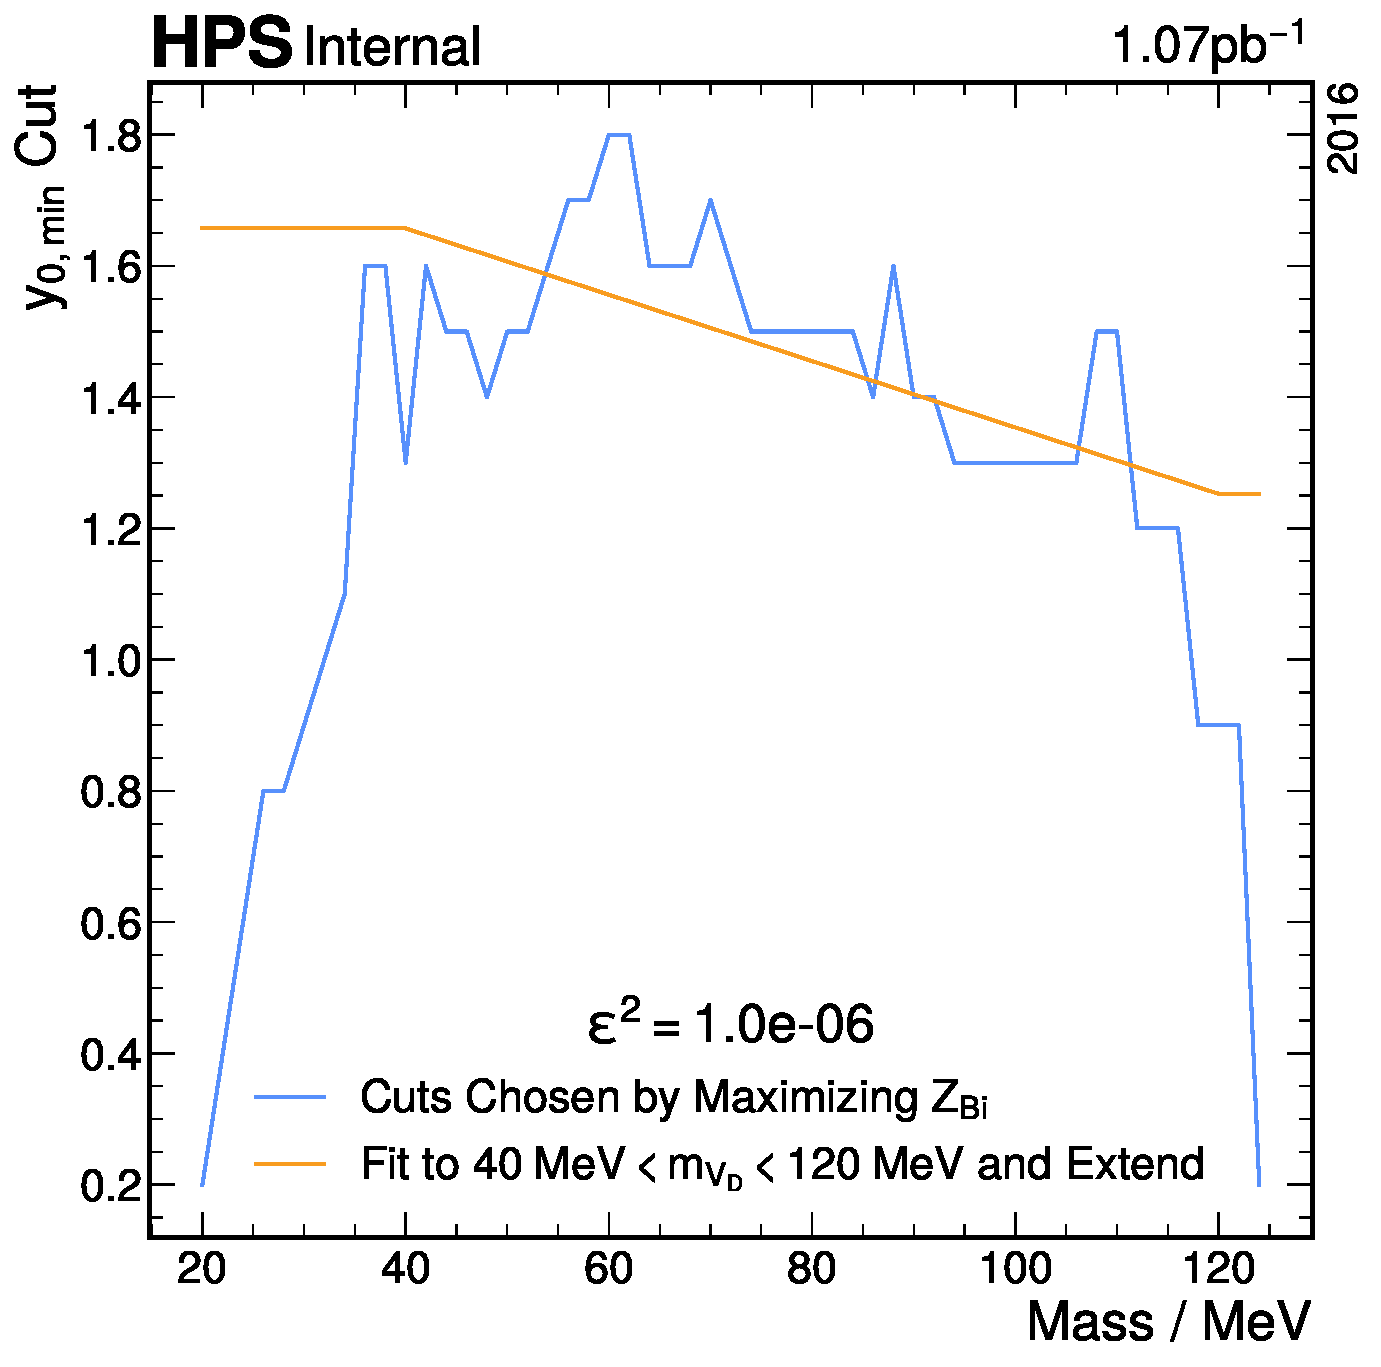
\includegraphics[width=\textwidth]{figures/hps/analysis/miny0-cut-after-others-fit-eps2-1e-6.pdf}
    \caption{%
      Values maximing the binomial signficance (blue) along with the linear fit and flat extension (orange).
    }
    \label{fig:miny0-opt:fit}
  \end{subfigure}
  \caption{%
    Binomail significance (left) being maximized after the \ac{vps}$< 4$ and
    \maxyzeroerr$<\qty{0.4}{\mm}$ cuts leading to cuts (right, blue) which are
    smoothed into a continuous function (right, orange) as described in the text.
  }
  \label{fig:miny0-opt}
\end{figure}

In summary, the following cuts developed for this analysis are
\begin{itemize}
  \item L1L2: In the vertex, one of the particles must have a hit in both sensors in
    layer 1 and layer 2 while the other must have a hit in both sensors in layer 2 and layer 3.
  \item Low Momentum Sum: $\qty{1.0}{\GeV} < $\Psum$ < \qty{1.9}{\mm}$
  \item Decay after Target: $z > z_\mathrm{target}$
  \item Vertex Projects Back to Beamspot: \ac{vps} $< 4$
  \item Good Vertical Resolution: \maxyzeroerr$< \qty{0.4}{\mm}$
\end{itemize}
A search for a statistically-significant excess of highly-displaced events
reconstructed within resolution of a specific mass is then performed at this point.
The sensitivity is estimated using two additional cuts.
\begin{itemize}
  \item Within Mass Window: $p_m < 2.8$
  \item Truly Displaced: \minyzero$> y_{0,\min}^\mathrm{cut}$
\end{itemize}
where
\begin{equation} \label{eq:miny0-cut-func}
  y_{0,\min}^\mathrm{cut}(m_\mathrm{reco}) = \begin{cases}
    A & m_\mathrm{reco} \leq \qty{40}{\MeV} \\
    B+Cm_\mathrm{reco} & \qty{40}{\MeV} < m_\mathrm{reco} < \qty{120}{\MeV} \\
    D & m_\mathrm{reco} \geq \qty{120}{\MeV} 
  \end{cases}
\end{equation}
and the parameters of this function are given in \cref{tab:miny0-cut-params}.

\begin{table}
  \centering
  \begin{tabular}{c|c}
    Parameter & Value \\ \hline
    $A$ & \qty{1.66}{\mm} \\
    $B$ & \qty{1.86}{\mm} \\
    $C$ & \qty{-5.1e-03}{\mm/\MeV} \\
    $D$ & \qty{1.25}{\mm}
  \end{tabular}
  \caption{Parameters for \cref{eq:miny0-cut-func}.}
  \label{tab:miny0-cut-params}
\end{table}

These selections lead to 88
highly-displaced events in data left which can be seen in \cref{fig:y0-cut-on-data}.
The total signal efficiency of this analysis as a function of reconstructed $z$
\cref{fig:signal-efficiency:l1l2} is of the same magnitude but slightly further displaced
than the L1L1 analysis \cref{fig:signal-efficiency:l1l1}.

\begin{figure}
  \centering
  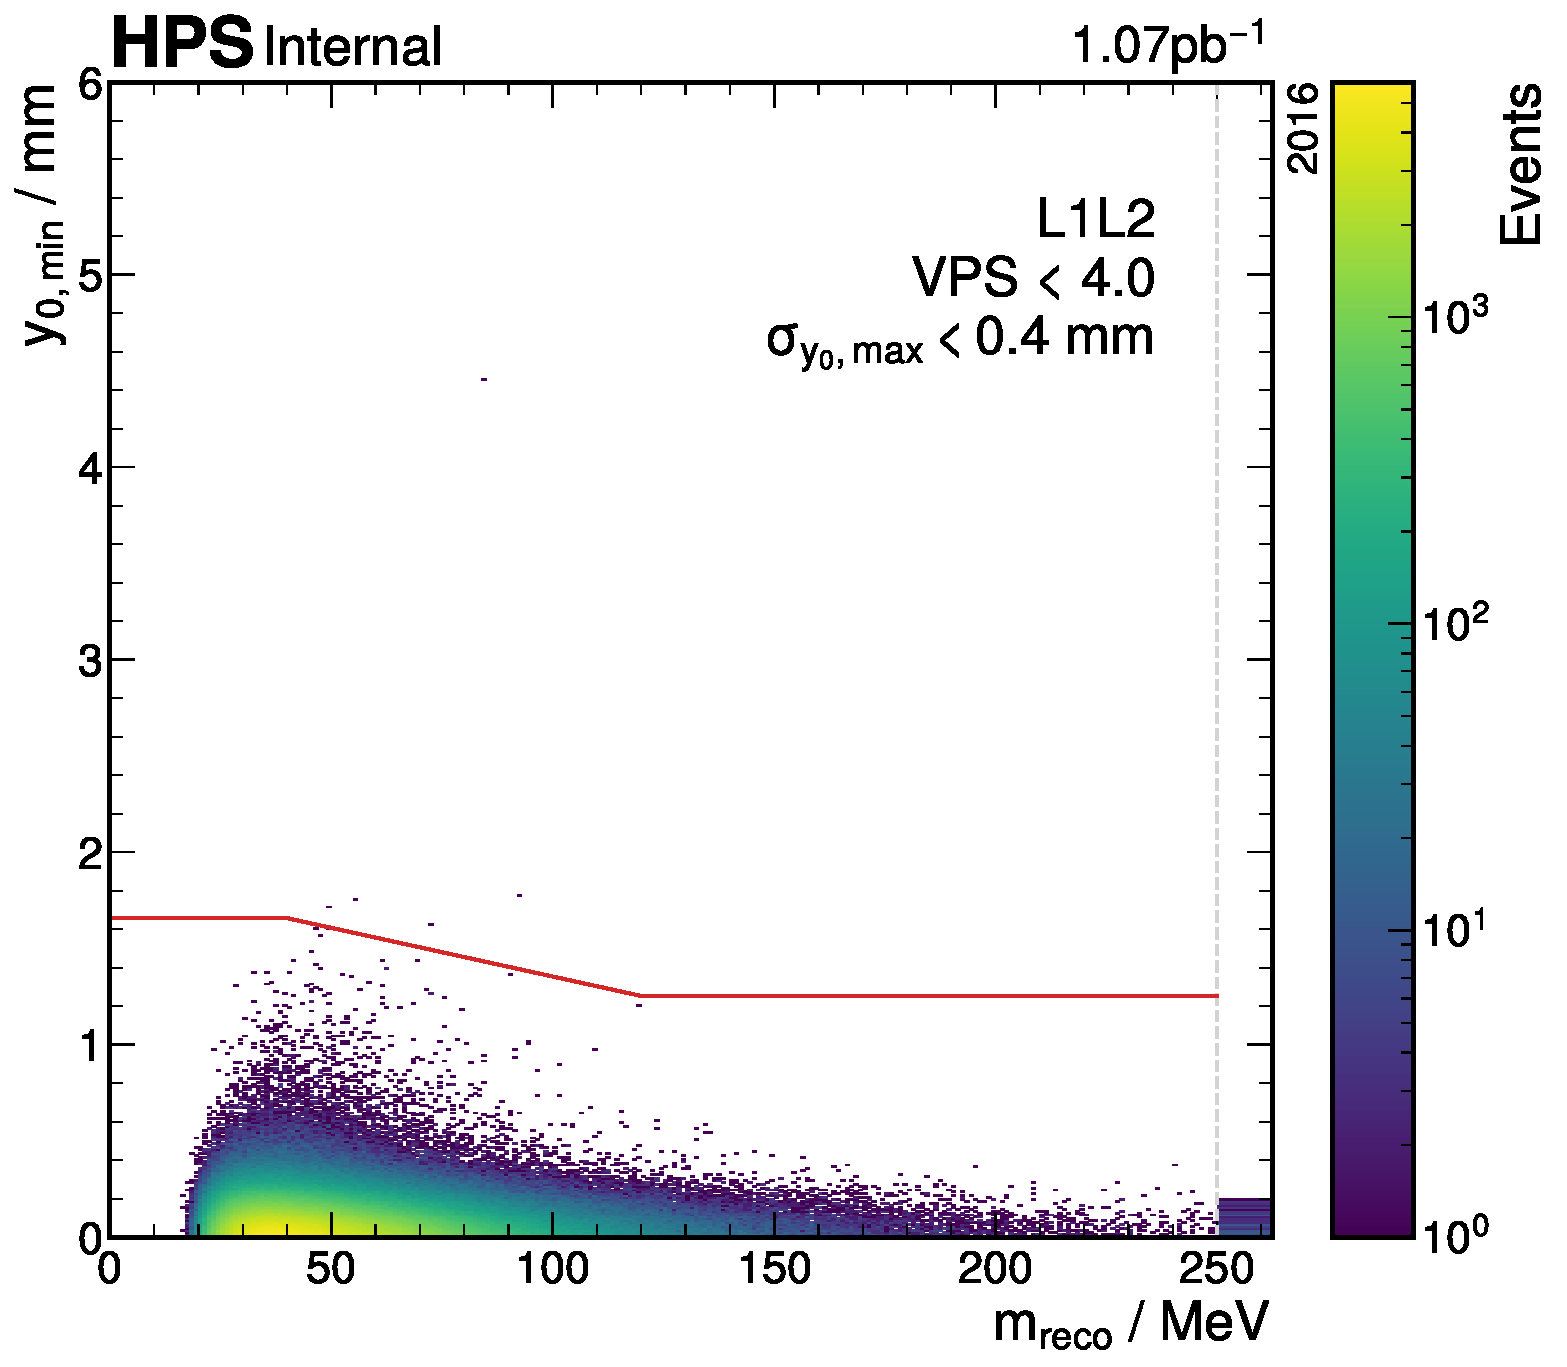
\includegraphics[width=0.5\textwidth]{figures/hps/analysis/results/y0-cut-on-data.pdf}
  \caption{\minyzero distribution for the 10\% data sample with the
  $y_{0,\min}^\mathrm{cut}$ function overlayed in red.}
  \label{fig:y0-cut-on-data}
\end{figure}

\begin{figure}
  \centering
  \begin{subfigure}{0.48\textwidth}
    \centering
    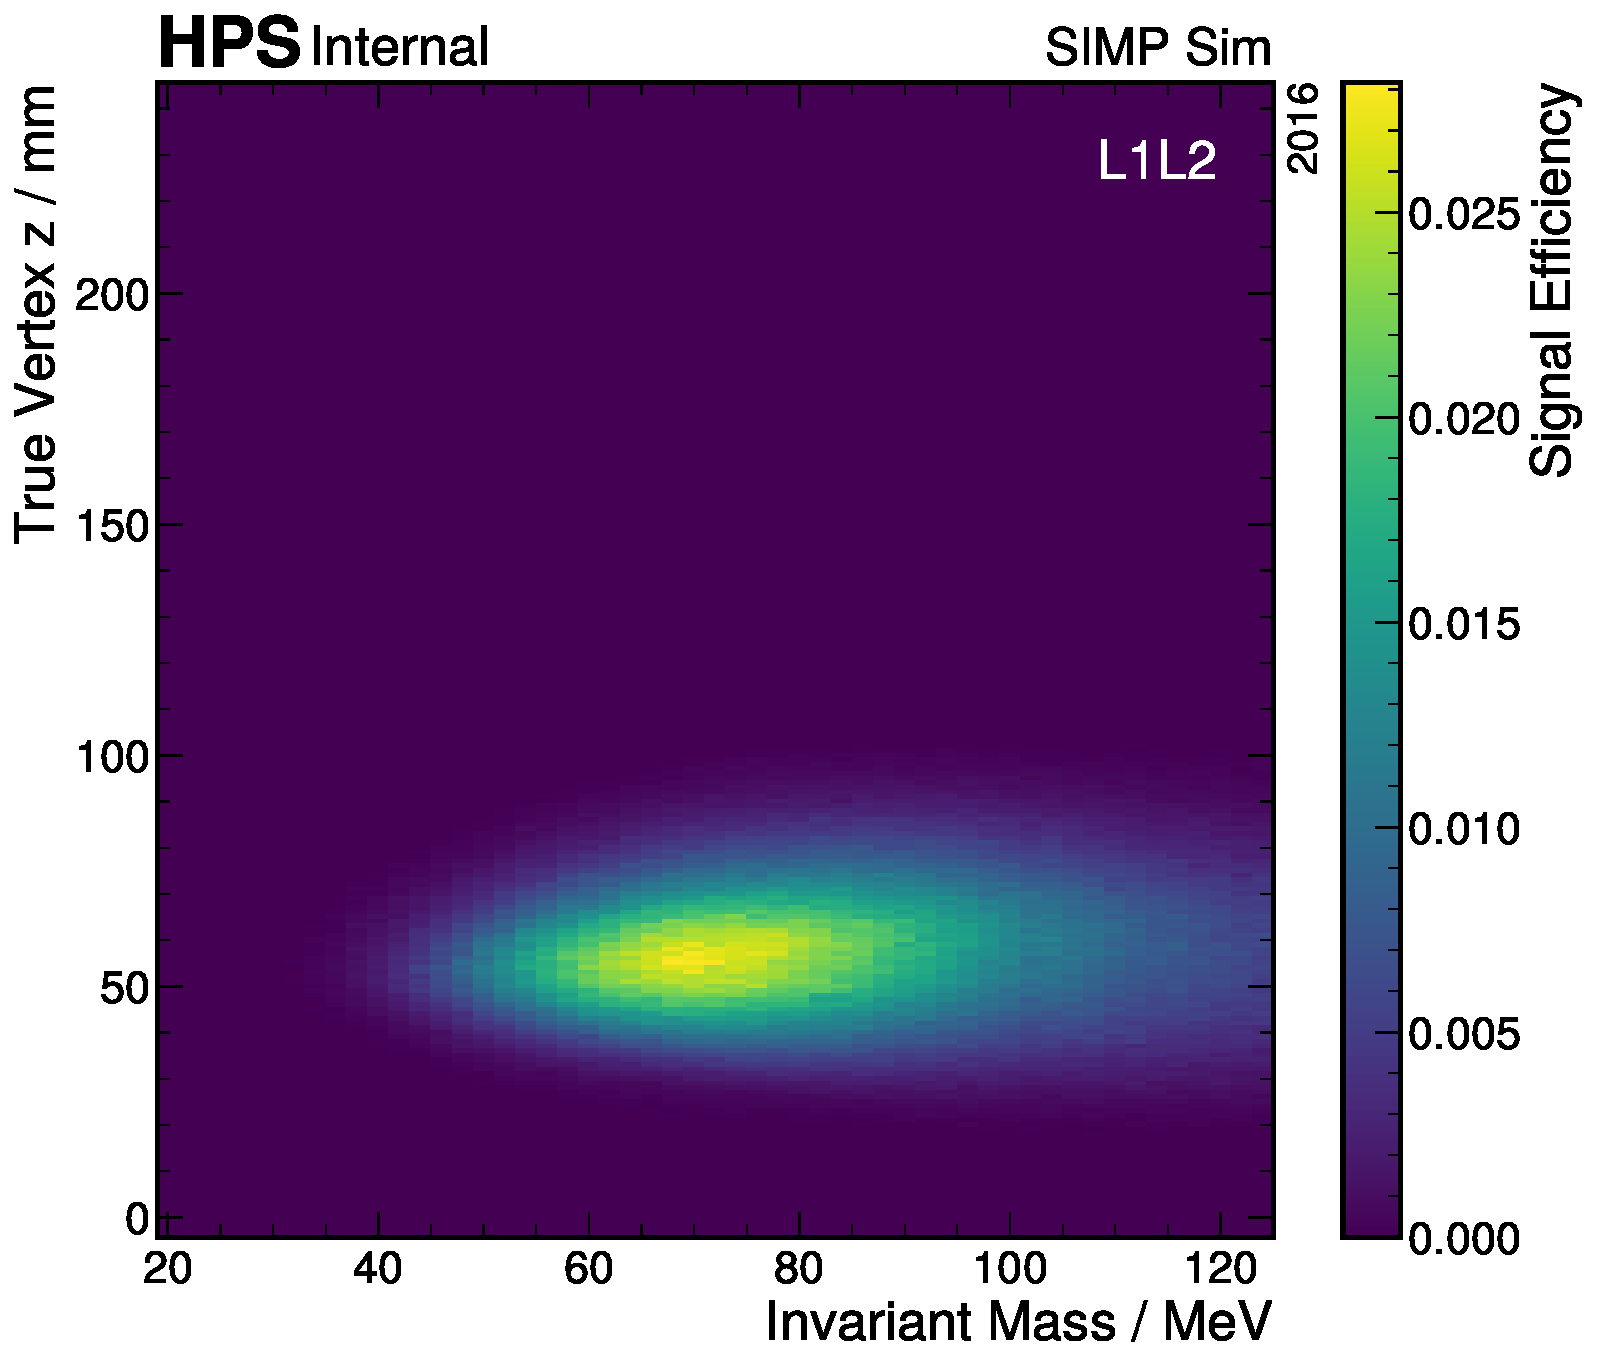
\includegraphics[width=\textwidth]{figures/hps/analysis/results/signal-efficiency.pdf}
    \caption{L1L2}
    \label{fig:signal-efficiency:l1l2}
  \end{subfigure}
  ~
  \begin{subfigure}{0.48\textwidth}
    \centering
    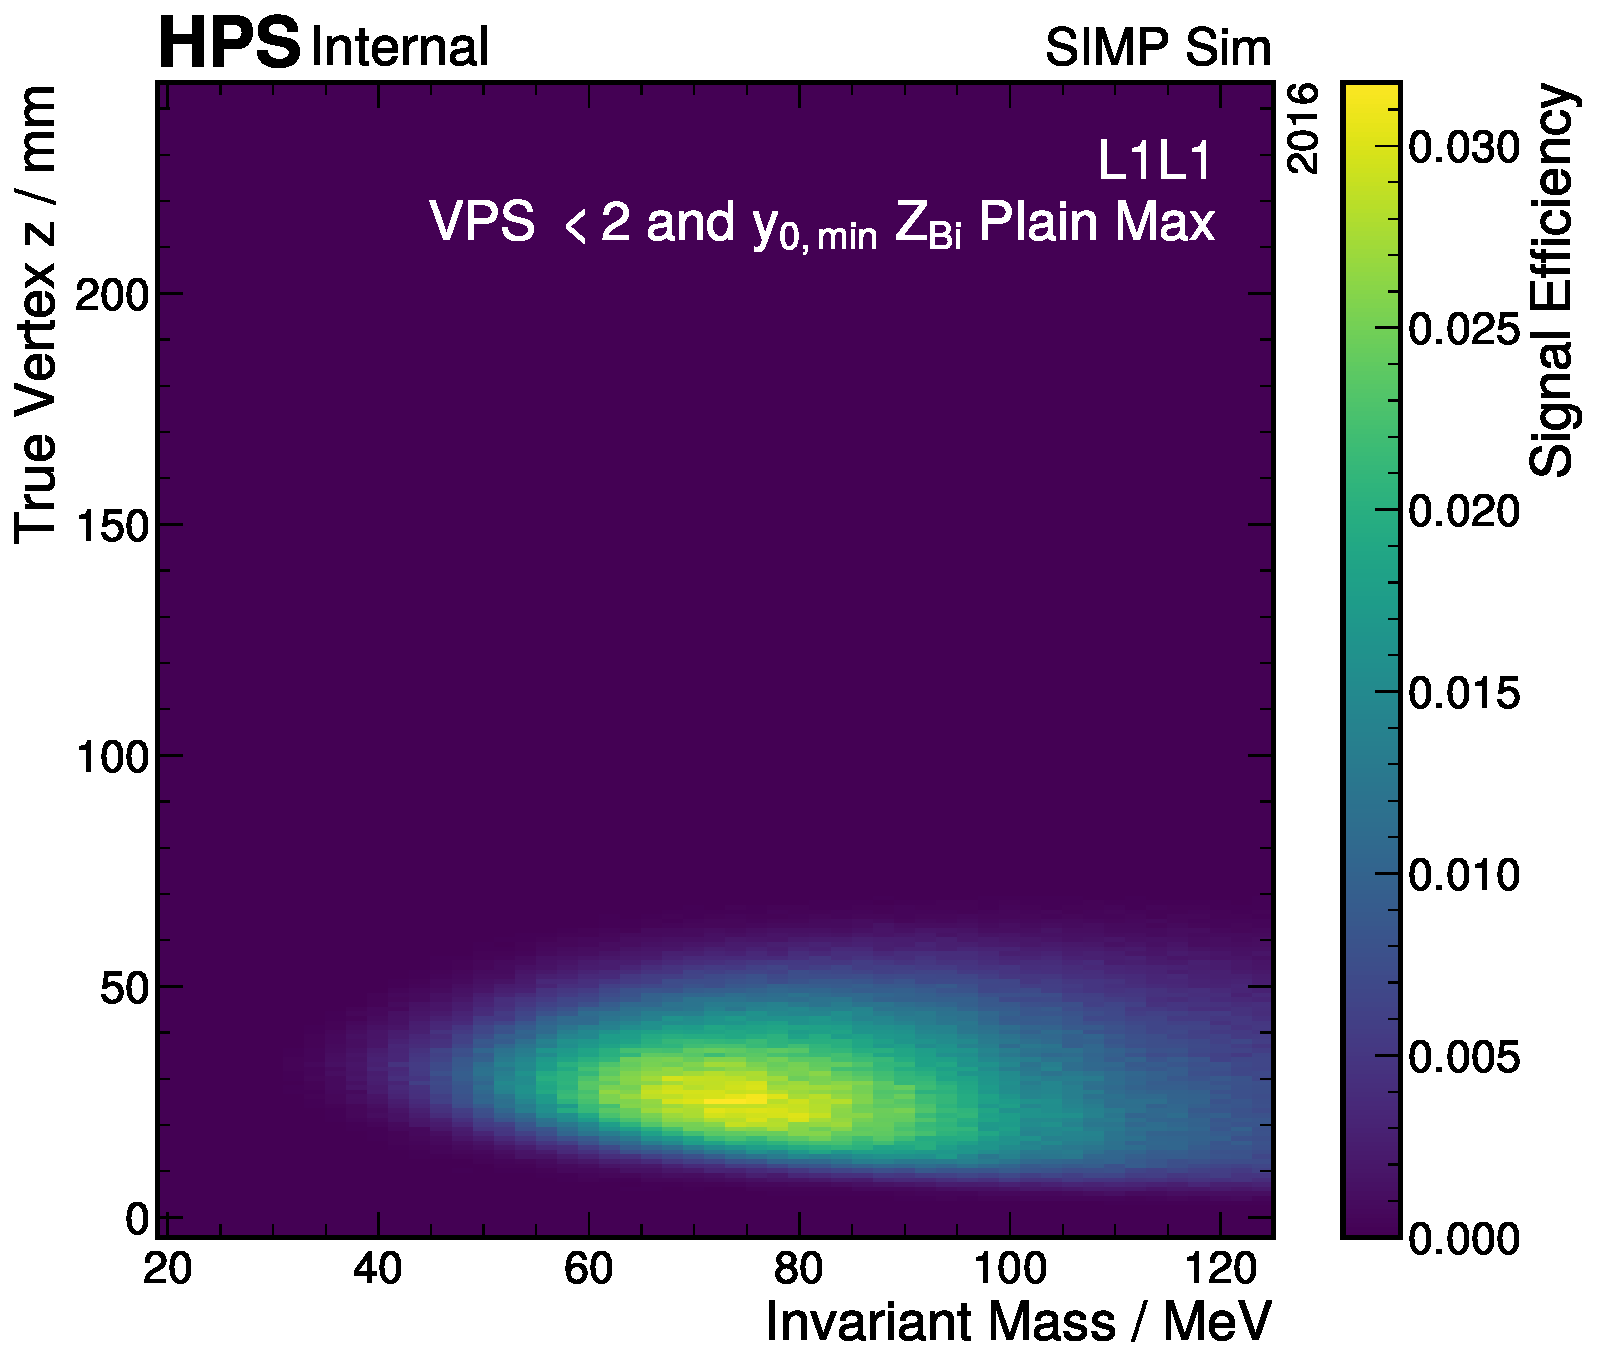
\includegraphics[width=\textwidth]{figures/hps/analysis/results/l1l1-signal-efficiency.pdf}
    \caption{L1L1}
    \label{fig:signal-efficiency:l1l1}
  \end{subfigure}
  \caption{Signal efficiency as a function of $z$ and mass scale $m_{V_D}$ for
  this analysis (left) and L1L1 (right).}
  \label{fig:signal-efficiency}
\end{figure}

\section{Results}
With the selection fixed, we can analyze the full sample of data without fear of
statistical bias.

\subsection{Search}
The first stage in this analysis is to perform the search for an excess of highly-displaced
events above what could be expected by the background.
The signal model we are searching for would have extra events that are both highly-displaced
and centered on a specific resonant mass; thus, the search is performed in the \minyzero -- $m_\mathrm{reco}$
space.
The expected number of background events is estimated using a variation of the ABCD technique
\todo[citation]{is there a citation for the ABCD technique?}
with two sidebands in mass (one below and one above the mass window in which we are searching)
and one sideband in \minyzero (one below the highly-dipsplaced region).
The sidebands in mass are defined in terms of the mass resolution of the detector $\sigma_m$
and the values defining these edges were optimized within the L1L1 analysis.
The sideband in \minyzero is defined such that the region within the mass window but
at lower displacment (Region C) has at least one thousand events within it to avoid signal contaminating
the background estimation.

\cref{tab:abcdef-regions} gives the definition of these regions.
\cref{fig:search:all} shows the search results comparing the expected number of events to the
observed along with a corresponding p-value estimated using ten thousand toy experiments.\footnote{
  Each toy experiment is constructed by sampling a toy values for regions C (normally distributed about actual value),
  B+D (normally distributed about actual value), and A+E (poisson distributed about actual value) and
  then re-calculating the expected number in region F. The number of toy experiments whose expected
  value in F was greater than or equal to the observed number in F divided by the total number of
  toy experiments is then our estimate p-value.
}
\cref{fig:search:min-p-val} shows an example of the search calculation using the mass point resulting
in the smallest p-value.

A few mass points had an excess of events observed within the signal region; however,
these excesses never exceeded a global significance of $3\sigma$ and thus are understood
as rare but normal statistical fluctuations.
The lowest p-value observed was \num{1.1e-03} which only barely exceeded $2\sigma$ global significance.

\begin{table}
  \centering
  \begin{tabular}{c|cc}
    Region & $m_\mathrm{reco}$ Range & \minyzero Range \\ \hline
    A & $(m_{V_D}-4.5\sigma_m,m_{V_D}-1.5\sigma_m)$ & $(y_{0,\min}^\mathrm{cut},\infty)$ \\
    B & $(m_{V_D}-4.5\sigma_m,m_{V_D}-1.5\sigma_m)$ & $(y_{0,\min}^\mathrm{floor},y_{0,\min}^\mathrm{cut})$ \\
    C & $(m_{V_D}-1.5\sigma_m,m_{V_D}+1.5\sigma_m)$ & $(y_{0,\min}^\mathrm{floor},y_{0,\min}^\mathrm{cut})$ \\
    D & $(m_{V_D}+1.5\sigma_m,m_{V_D}+4.5\sigma_m)$ & $(y_{0,\min}^\mathrm{floor},y_{0,\min}^\mathrm{cut})$ \\
    E & $(m_{V_D}+1.5\sigma_m,m_{V_D}+4.5\sigma_m)$ & $(y_{0,\min}^\mathrm{cut},\infty)$ \\
    F & $(m_{V_D}-1.5\sigma_m,m_{V_D}+1.5\sigma_m)$ & $(y_{0,\min}^\mathrm{cut},\infty)$
  \end{tabular}
  \caption{%
    Region definitions for use in background estimation via sidebands.
    Region F is the signal region in which we are searching for an excess.
    $m_{V_D}$ is the mass point we are searching for,
    $\sigma_m$ is the detector mass resolution evaluated at $m_{V_D}$,
    $y_{0,\min}^\mathrm{cut}$ is the optimized cut value evaluated at $m_{V_D}$,
    and $y_{0,\min}^\mathrm{floor}$ is the maximum value of $y_{0,\min}$ such that region C
    has at least one thousand events in it.
  }
  \label{tab:abcdef-regions}
\end{table}

\begin{figure}
  \centering
  \begin{subfigure}{0.48\textwidth}
    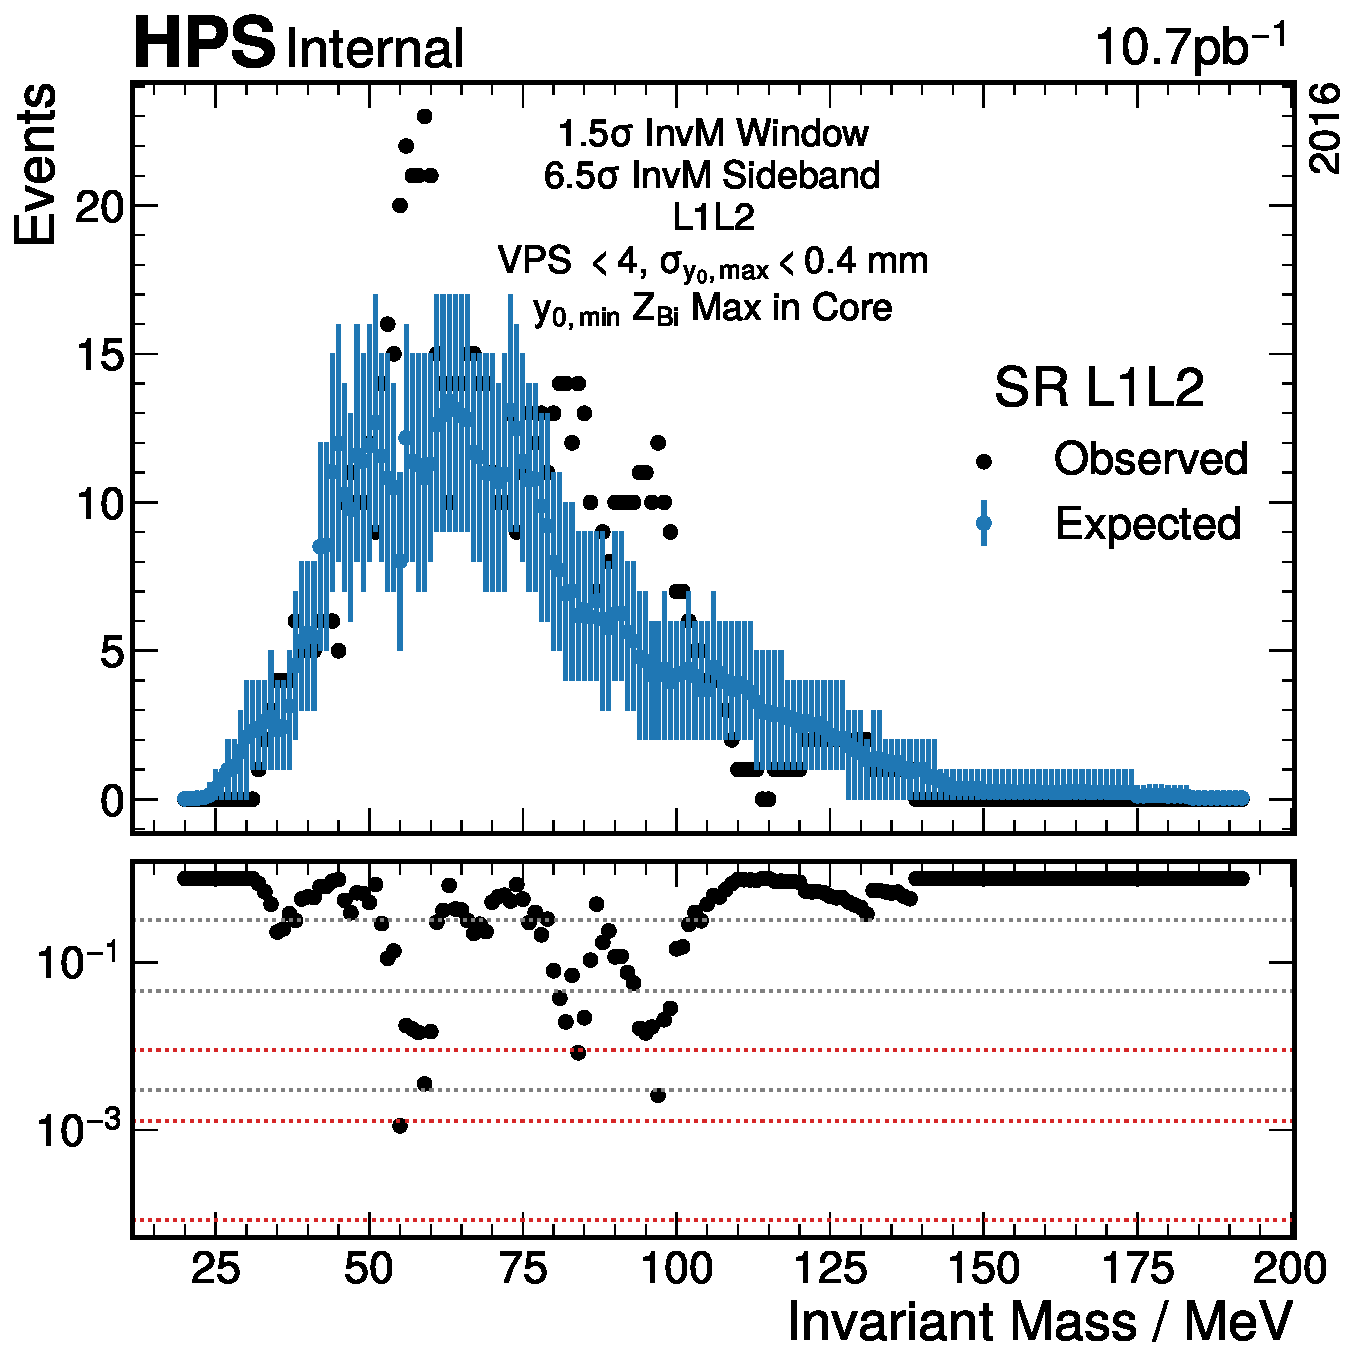
\includegraphics[width=\textwidth]{figures/hps/analysis/results/search.pdf}
    \caption{Expected and observed events (top) with their p-values (bottom).}
    \label{fig:search:all}
  \end{subfigure}
  ~
  \begin{subfigure}{0.48\textwidth}
    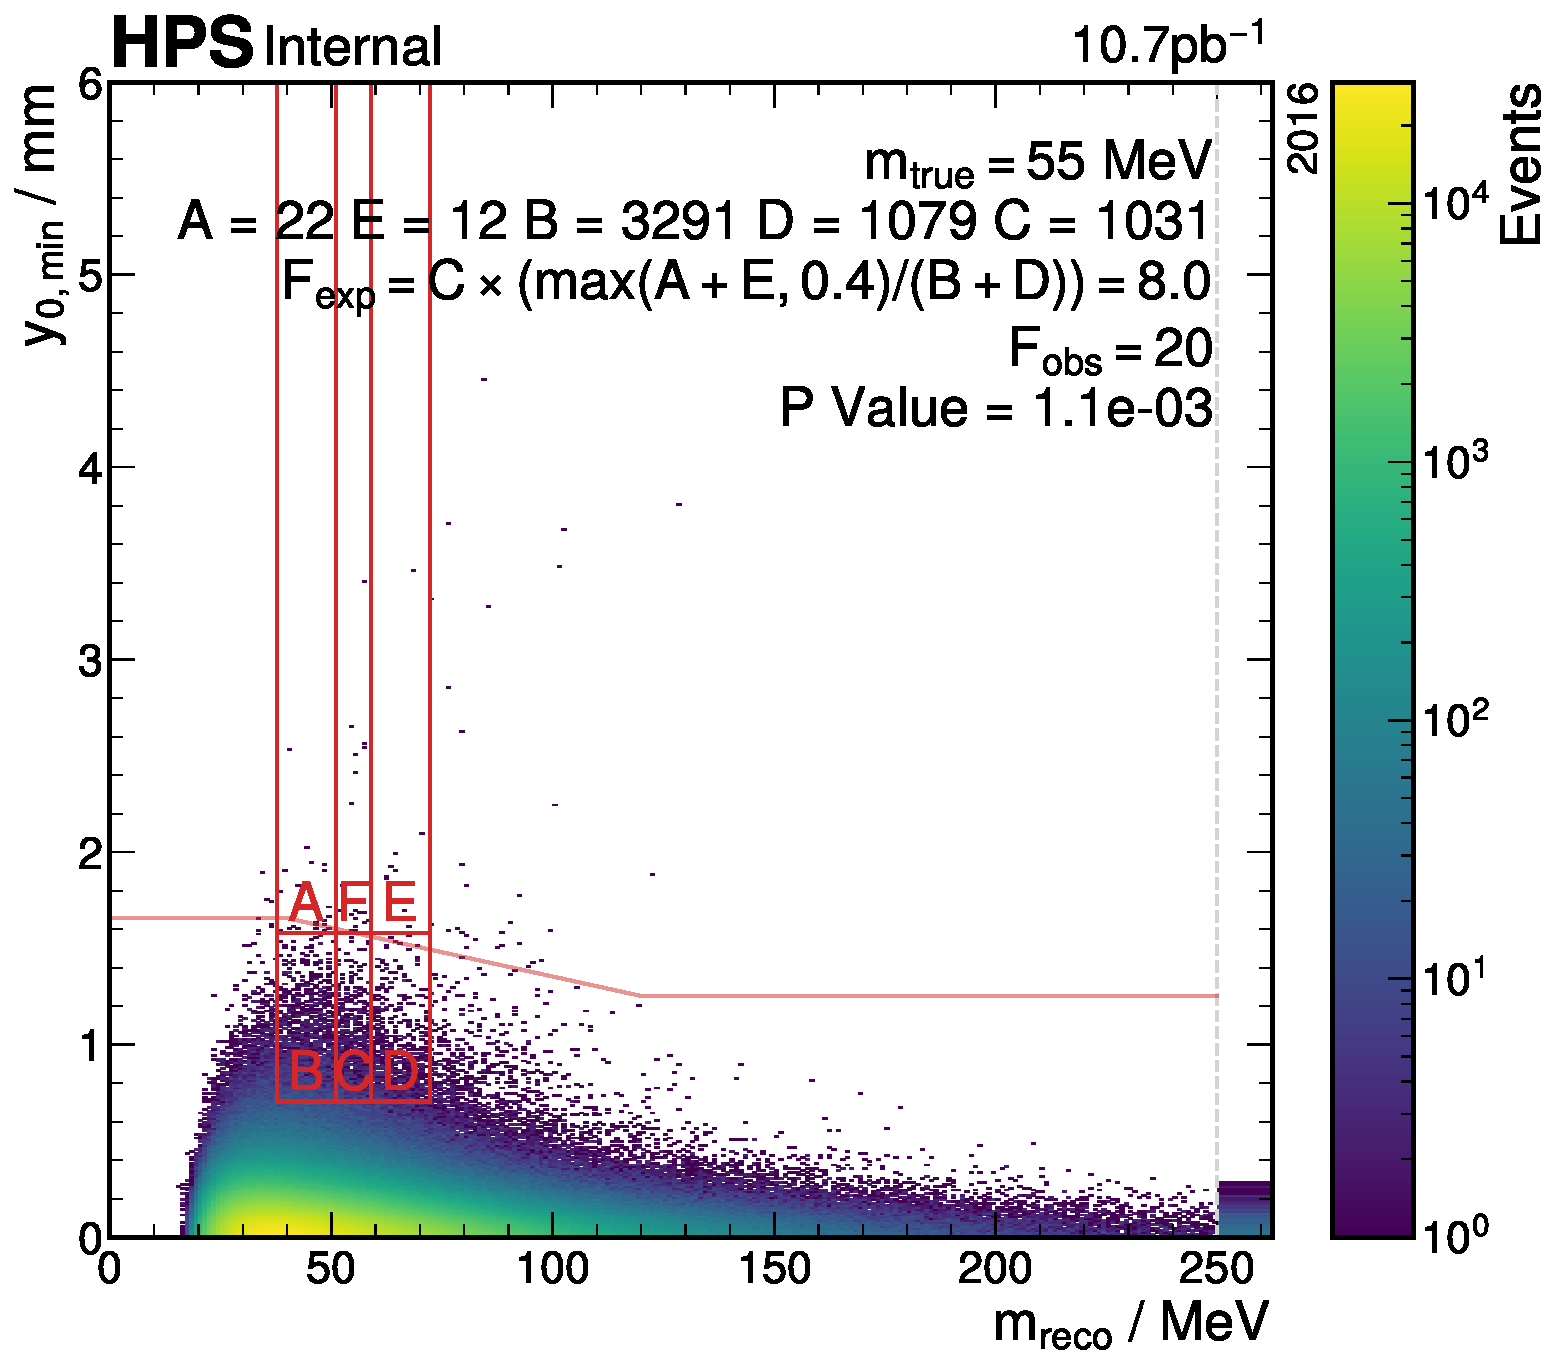
\includegraphics[width=\textwidth]{figures/hps/analysis/results/search-min-p-val.pdf}
    \caption{Search calculation yielding the minimum p-value
    (with $y_{0,\min}^\mathrm{cut}$ in light red).}
    \label{fig:search:min-p-val}
  \end{subfigure}
  \caption{Search results on 10\% of the data.}
  \label{fig:search}
\end{figure}

\subsection{Sensitivity and Exclusion}
With no statistically-significant excess observed, we can then move towards estimating the sensitivity of
the analysis and then to exclude certain regions of parameter space.
The sensitivity estimate is rather simple; just a ratio between the expected signal yield
and the maximum signal yield allowed by the observed data distribution.
\cref{sec:hps:signal-yield} already described the expected signal calculation used here
as well as previously within the selection optimization.
\cref{fig:hps-signal-yield:expected} shows the final expected signal yield for this selection
using the full data sample.
The maximum signal yield allowed is calculated using the \ac{oim} \cite{yellin-oim:2002}
which leverages the differing shape between signal and background and allows for the presence
of unknown background to alter its scale.
The \ac{oim} result is shown in \cref{fig:hps-signal-yield:allowed}.

\cref{fig:sensitivity} shows the sensitivity for both this analysis of L1L2 and the L1L1 analysis
for comparison along with a contour drawn where the sensitivity equals one after being suppressed
by potential systematic errors.

This contour encloses the excluded parameter space where the expected yield exceeds what is allowed.
In this region of parameter space, BaBar\cite{babar-2017}
excluded the parameters above $\epsilon^2 = 10^{-6}$, so this analysis does not exclude new parameter space.
Nevertheless, this analysis was the first of its kind (low-\Psum) for \ac{hps} and thus
opens the door to further refinement and investigation with later and larger datasets.

\begin{figure}
  \centering
  \begin{subfigure}{0.48\textwidth}
    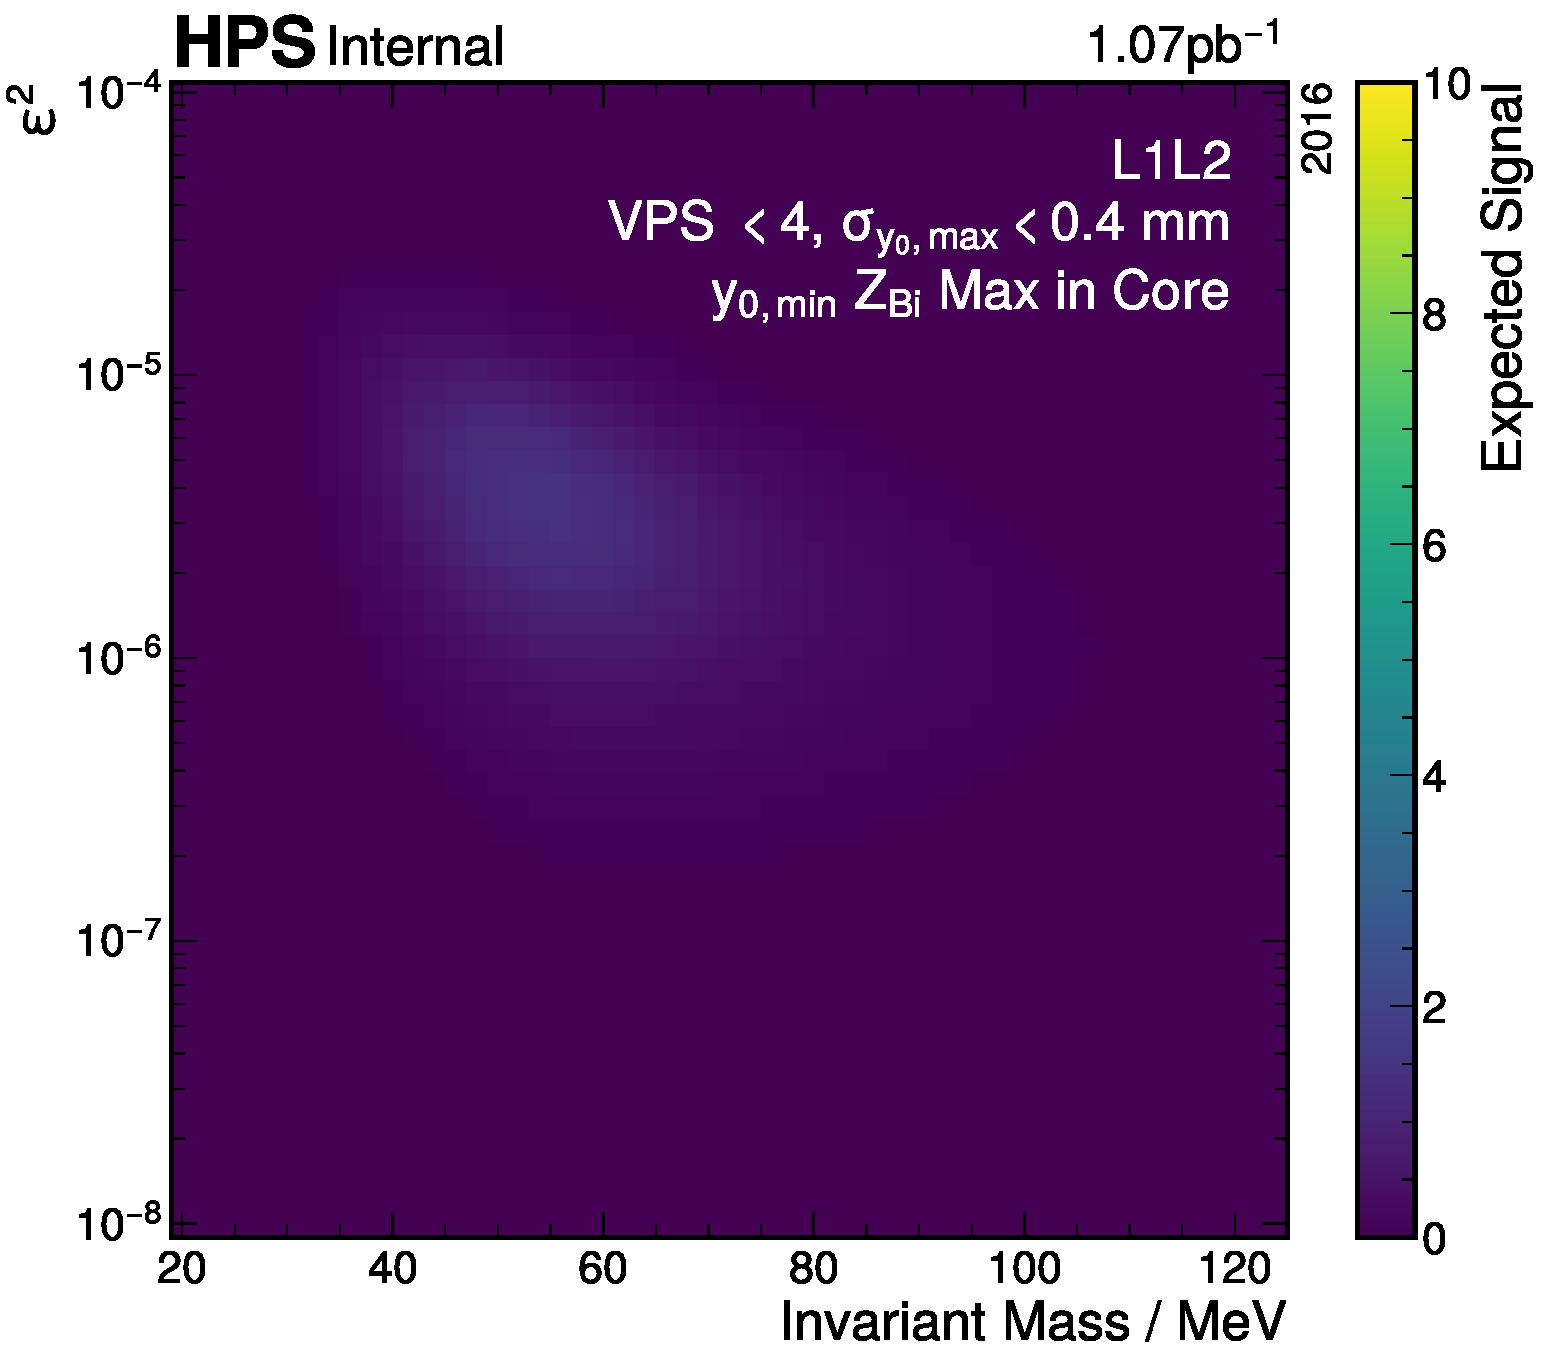
\includegraphics[width=\textwidth]{figures/hps/analysis/results/expected-signal.pdf}
    \caption{Expected}
    \label{fig:hps-signal-yield:expected}
  \end{subfigure}
  ~
  \begin{subfigure}{0.48\textwidth}
    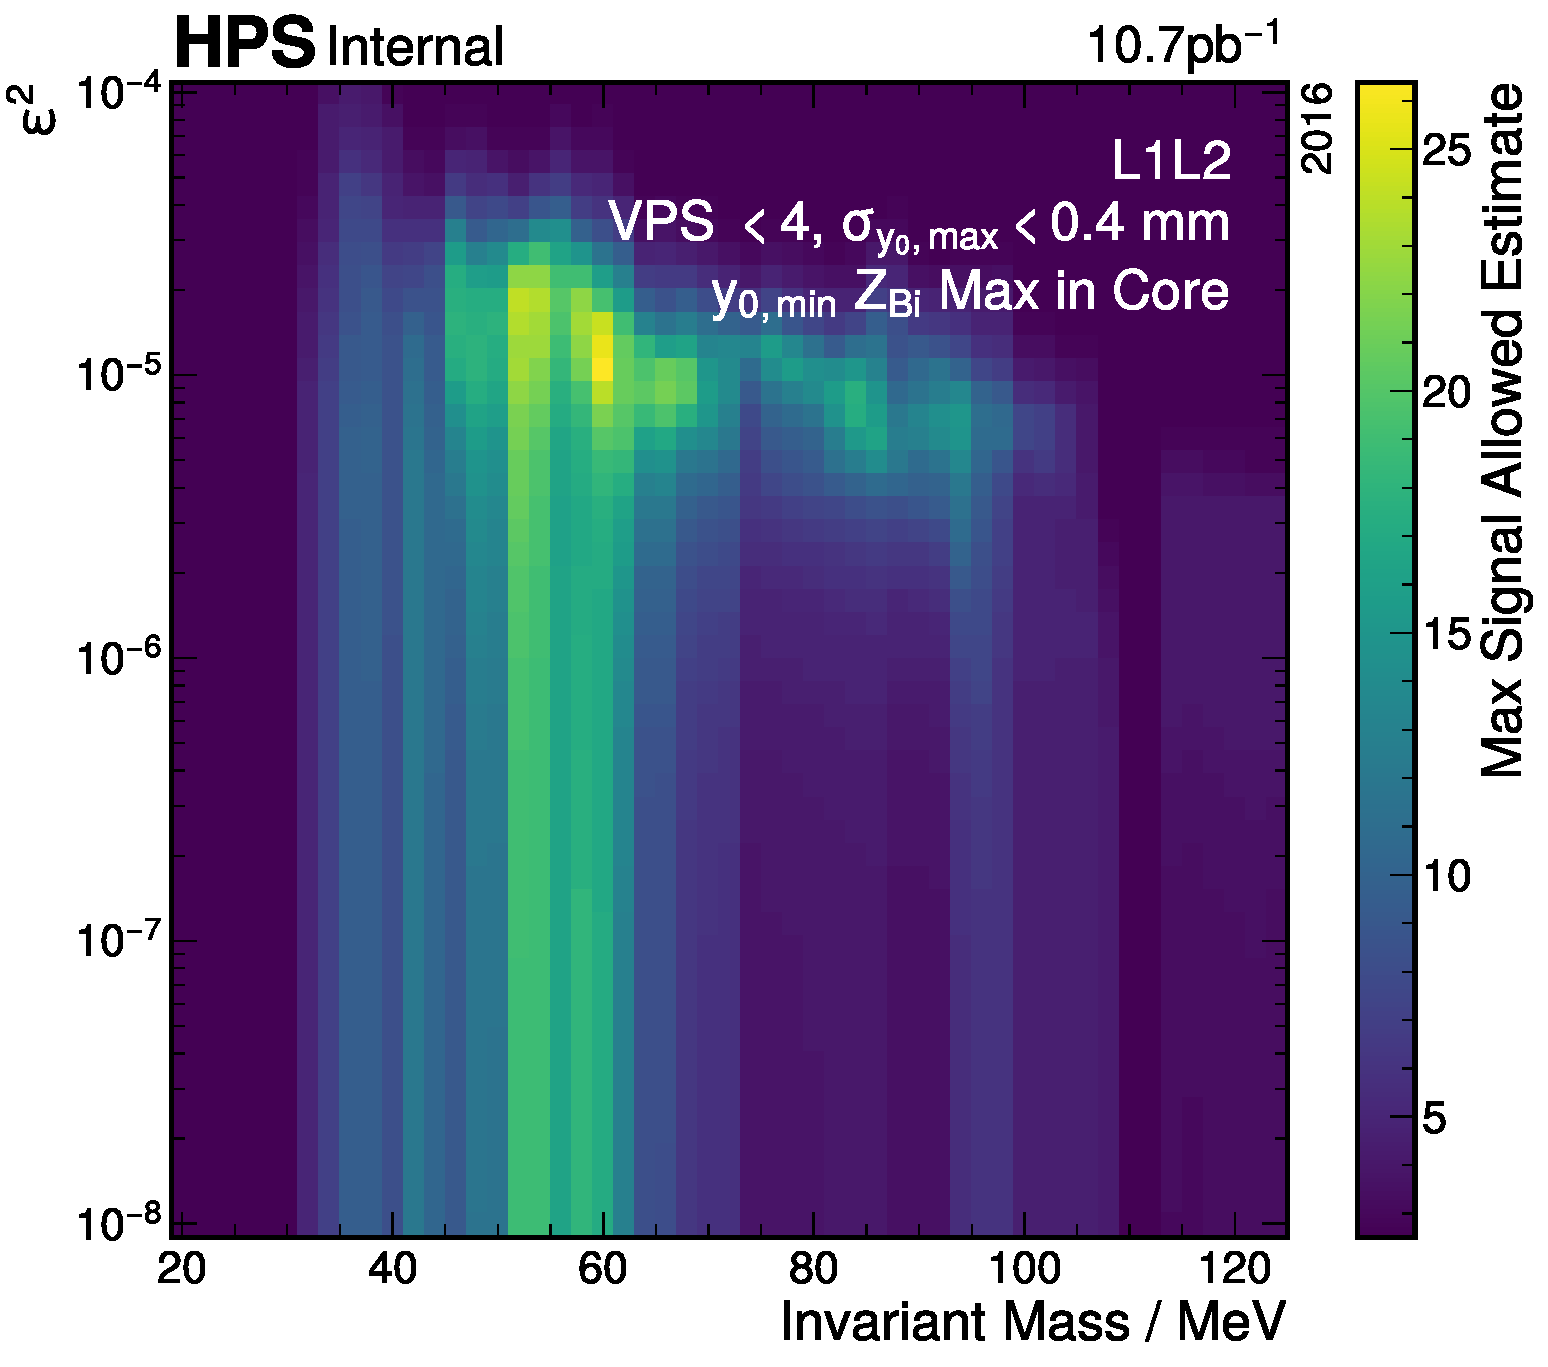
\includegraphics[width=\textwidth]{figures/hps/analysis/results/max-signal-allowed.pdf}
    \caption{Maximum Allowed}
    \label{fig:hps-signal-yield:allowed}
  \end{subfigure}
  \caption{Signal yield for the L1L2 reconstruction category with the described cuts
  showing the theoretical expecation (left) and the maximum allowed (right) derived
  using the \ac{oim}.}
  \label{fig:hps-signal-yield}
\end{figure}

\begin{figure}
  \centering
  \begin{subfigure}{0.48\textwidth}
    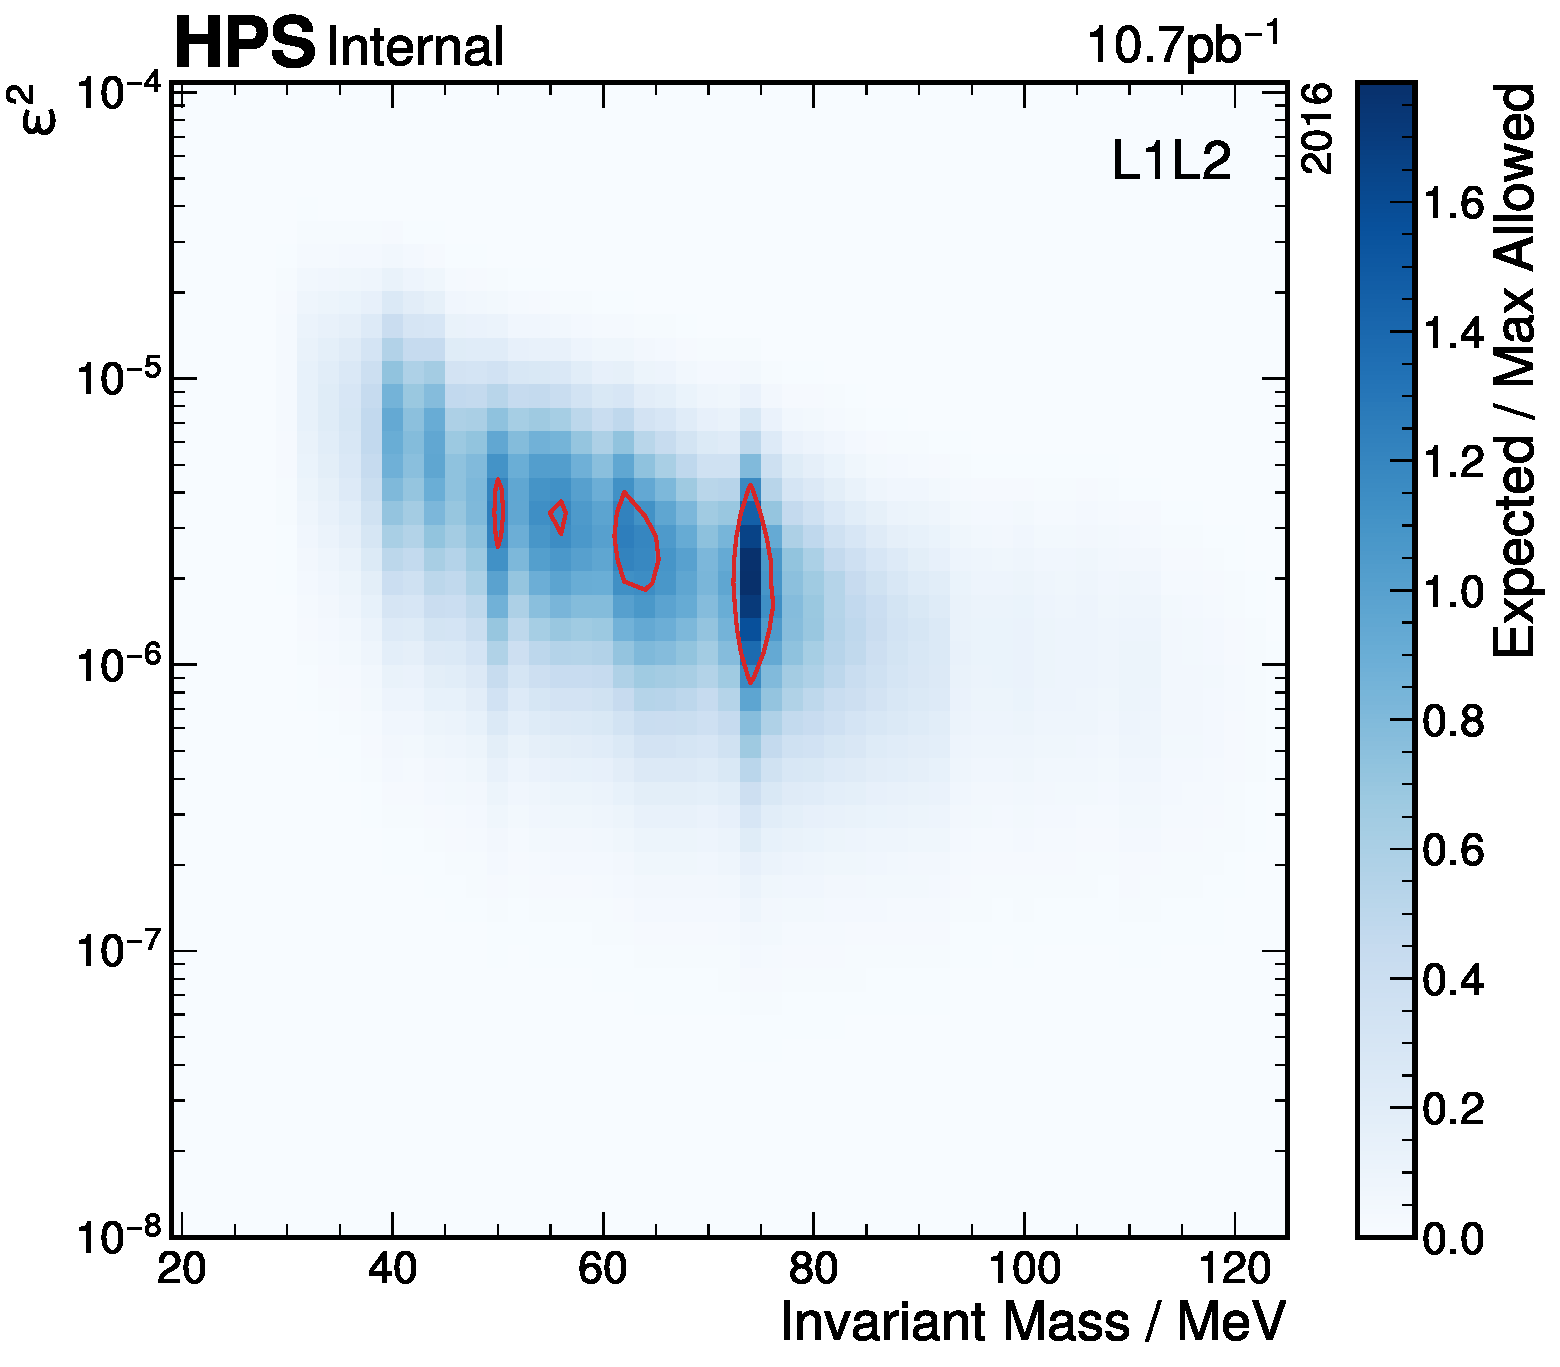
\includegraphics[width=\textwidth]{figures/hps/analysis/results/exclusion-estimate.pdf}
    \caption{L1L2}
    \label{fig:sensitivity:l1l2}
  \end{subfigure}
  ~
  \begin{subfigure}{0.48\textwidth}
    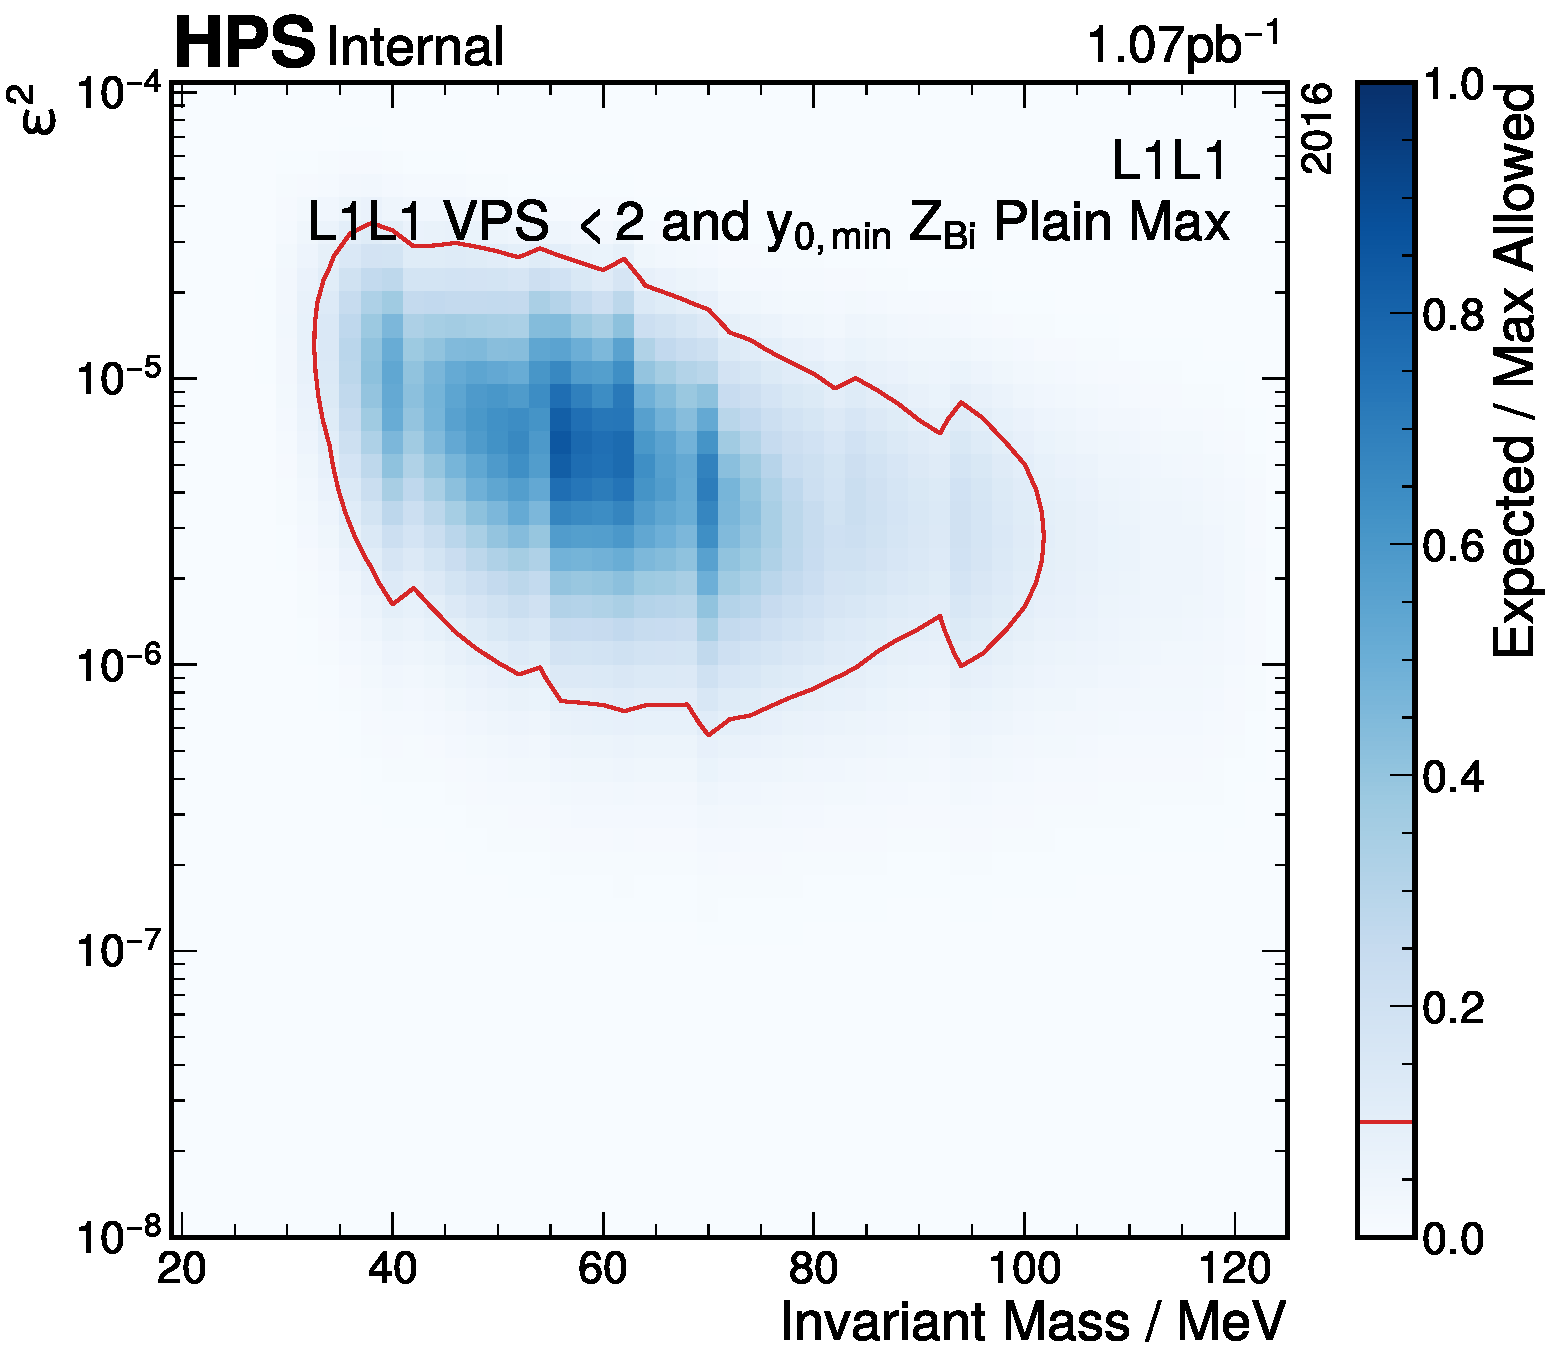
\includegraphics[width=\textwidth]{figures/hps/analysis/results/l1l1-exclusion-estimate.pdf}
    \caption{L1L1}
    \label{fig:sensitivity:l1l1}
  \end{subfigure}
  \caption{Sensitivity of this analysis with contour drawn including systematic errors
  surpressing the expected signal yield.}
  \label{fig:sensitivity}
\end{figure}
